%!TEX program = pdflatex
%----------------------------------------------------------------------------------------------------------------------
% Author: Jonas Nygaard Eriksen
% Encoding: UTF8
% LaTeX File for "Expected Business Conditions and Bond Risk Premia" 
% Last modified: December, 2015
%----------------------------------------------------------------------------------------------------------------------
% PREAMBLE
%----------------------------------------------------------------------------------------------------------------------

% Require the nag package to warn about obsolete stuff
\RequirePackage[l2tabu,orthodox]{nag}

% Formatting JFQA requirements
\documentclass[12pt,letterpaper,leqno,doublespacing]{article}
\usepackage[left=1in,right=1in,top=1in,bottom=1in]{geometry}
\usepackage{setspace}  
\usepackage{footmisc}
\usepackage{titlesec}
\renewcommand{\footnotelayout}{\doublespacing}
\setlength{\footnotesep}{0.5cm}
\titleformat{\section}[block]{\Large\bfseries}{\thesection.}{1em}{}
\titleformat{\subsection}[block]{\large\bfseries}{\thesubsection.}{1em}{}
\renewcommand{\thesection}{\Roman{section}}
\renewcommand{\thesubsection}{\Alph{subsection}}
\renewcommand{\thesubsubsection}{\Alph{subsection}.\arabic{subsubsection}}

% Setting document class, font, font size, and bibliography op tions
% \documentclass[12pt,a4paper,onecolumn,oneside,notitlepage]{article}
% \usepackage[left=2.5cm,right=2.5cm,top=2.5cm,bottom=2.5cm]{geometry}
% \usepackage[onehalfspacing]{setspace}

% Setting bibliography and typography options
\usepackage[longnamesfirst]{natbib}
\usepackage[english]{babel}
\usepackage[utf8]{inputenc}
\usepackage{eucal}
\usepackage[T1]{fontenc}
\usepackage{hyphenat}
\usepackage{microtype}
\usepackage{verbatim}

% Loading math packages
\usepackage{amsmath}
\usepackage{amsfonts}
\usepackage{amssymb}
\usepackage{amsthm}

% Loading tables and figures packages
\usepackage{makeidx}
\usepackage{tabularx}
\usepackage{graphicx}
\usepackage{epstopdf}
\usepackage{booktabs}
\usepackage{lscape}
\usepackage{longtable}
\usepackage{seqsplit}
\usepackage{rotating}
\usepackage{multicol}

% Loading auxiliary packages
\usepackage{soul}
\usepackage{blindtext}
\usepackage{appendix}

% Setting caption options
\usepackage{caption}
\usepackage{subcaption}
\captionsetup{
    labelfont = bf,
    labelsep = colon
}

% Setting coloring of links and references
\usepackage{hyperref}
\usepackage{xcolor}
\definecolor{au_blue}{RGB}{5,61,115}
\definecolor{navy_blue}{RGB}{0,0,128}
\definecolor{dark_red}{RGB}{153,0,0}
\definecolor{stylish_brown}{RGB}{188,90,100}
\definecolor{dark_orange}{RGB}{233,129,45}
\hypersetup{
    colorlinks=true,
    breaklinks=true,
    bookmarksnumbered=true,
    bookmarksopen=true,
    bookmarksdepth=2,
    citecolor=dark_red,
    linkcolor=dark_red,
    urlcolor=navy_blue,
    pdftitle={Expected Business Conditions and Bond Risk Premia},
    pdfauthor={Jonas Nygaard Eriksen}
}

% Setting up values for table creation
\renewcommand{\arraystretch}{0.95}
\newcolumntype{Y}{>{\centering\arraybackslash}X}
\newcolumntype{Z}{>{\raggedright\arraybackslash}X}

% SETTING BIBLIOGRAPHY PROPERTIES
\setlength{\bibsep}{0.1pt plus 0.3ex}

%----------------------------------------------------------------------------------------------------------------------
% FRONT MATTER
%----------------------------------------------------------------------------------------------------------------------

\begin{document}

% Defining title and footnotes
\pagenumbering{Alph}
\newcommand{\mytitle}{\textbf{\Large{Expected Business Conditions and Bond Risk Premia}}}
\renewcommand{\refname}{References}
\long\def\symbolfootnote[#1]#2{\begingroup\def\thefootnote{\fnsymbol{footnote}}\footnote[#1]{#2}\endgroup}

% Setting up custom title page
\begin{titlepage}

    \thispagestyle{empty}
    \setlength{\parindent}{0cm}
    \begin{center}

        \small
        \renewcommand{\thefootnote}{\fnsymbol{footnote}}

        \vspace*{4cm} 
        \mytitle\symbolfootnote[1]{
            I am grateful to Stig Vinther Møller, Maik Schmeling, an anonymous referee, and seminar participants at Aarhus University and CREATES and the 2015 Nordic Econometric Meeting in Helsinki for helpful comments and suggestions. The author acknowledge support from CREATES - Center for Research in Econometric Analysis of Time Series (DNRF78), funded by the Danish National Research Foundation
        }

        \vspace*{3cm}
        \textbf{\normalsize{
            Jonas Nygaard Eriksen}\symbolfootnote[7]{CREATES, Department of Economics and Business Economics, Aarhus University, Fuglesangs All{\'e} 4, DK-8210 Aarhus V, Denmark. Tel.: +45 87165321. E-mail: \href{mailto:jeriksen@econ.au.dk}{jeriksen@econ.au.dk}.
            }
        }

        \vspace{1.2cm}
        {
            \normalsize  
            \vspace{1.5cm}
            This version: \today
        }
        \clearpage
        \thispagestyle{empty}
        \vspace*{2cm}
        \mytitle
        \vspace*{0.5cm}
        \begin{singlespace}
            \begin{abstract}
                \noindent This paper studies the predictability of bond risk premia by means of expectations to future business conditions using survey forecasts from the Survey of Professional Forecasters. We show that expected business conditions consistently affect excess bond returns and that the inclusion of expected business conditions in standard predictive regressions improve forecast performance relative to models using information derived from the current term structure or macroeconomic variables. The results are confirmed in a real-time out-of-sample exercise, where the predictive accuracy of the models is evaluated both statistically and from the perspective of a mean-variance investor that trades in the bond market. \\\bigskip
                \noindent\textbf{Keywords:} Bond risk premia, expected business conditions, predictability, economic value, expectations hypothesis, time-varying risk premia\\\medskip
                \noindent\textbf{JEL Classification:} E43, E44, E47, G11, G12. \\\bigskip
                \noindent\textbf{This version:} \today
            \end{abstract}
        \end{singlespace}
    \end{center}        
\end{titlepage}

%----------------------------------------------------------------------------------------------------------------------
% INTRODUCTION
%----------------------------------------------------------------------------------------------------------------------

\clearpage
\setcounter{page}{1}
\pagenumbering{arabic}
\section{Introduction}\label{Sec:e_introduction}
There is mounting evidence that the risk premia required by investors for holding Treasury bonds contain a time-varying and predictable component. One strand of research relates such variations to forward spreads \citep{FamaBliss1987,Fama2006}, yield spreads \citep{KeimStambaugh1986,CampbellShiller1991}, and forward rates \citep{CochranePiazzesi2005,DahlquistHasseltoft2013,Zhu2015}, whereas more recent studies link the predictable component to factors whose variations lie outside the span of current yields. Existing research within this strand has uncovered a wide array of factors including jump risk \citep{WrightZhou2009}, option prices \citep{AlmeidaGravelineJoslin2011}, and macroeconomic variables \citep{Ilmanen1995,Moench2008,CooperPriestley2009,LudvigsonNg2009,Wright2011,FaveroNiuSala2012,JoslinPriebschSingleton2014,ZhouZhu2015}. 

While existing studies mainly rely on information in the current term structure and business environment to explain variations in the predictable component of bond risk premia, our study takes a forward-looking perspective by studying the link between expected business conditions and bond risk premia using survey forecasts from the \emph{Survey of Professional Forecasters} (SPF). Albeit empirical studies frequently conclude that macroeconomic fundamentals carry information about bond risk premia not already captured by the yield curve, they rarely account for issues with publication lags and data revisions in macroeconomic time series. As recently demonstrated by \cite{GhyselsHoranMoench2014}, such features may drive a wedge between the factor spaces spanned by latent common factors extracted from a panel of revised and non-revised data, respectively, implying that a sizable fraction of the predictability documented by \cite{LudvigsonNg2009} may largely be driven by revision and publication lag components that are unavailable to an investor in real-time. Survey forecasts, as a result, provide an ideal data source for studying the predictability of bond risk premia as they are model-free, available in real-time, and not subject to subsequent revisions \citep{AmatoSwanson2001,CroushoreStark2001,PesaranTimmermann2005}. Moreover, the use of survey forecasts allows us to investigate if macroeconomic expectations influence future bond risk premia as suggested by, among others, \cite{ChenRollRoss1986}, \cite{FamaFrench1989}, \cite{Barro1990}, \cite{Fama1990}, and \cite{FersonHarvey1991}. 

Using the SPF survey forecasts, we investigate empirically whether expected business conditions are related to one-year ahead variations in bond risk premia and, secondly, whether expected business conditions contain information orthogonal to current business conditions and yield curve information. Our findings suggest that excess bond returns are indeed predictable by expected business conditions. In particular, we find that expected business conditions are able explain about $20\%$ of the one-year ahead variation in bond risk premia. Consistent with recent research, we find the majority of the informational content in expected business conditions to lie outside the span of contemporaneous yields \citep{Duffee2011,JoslinPriebschSingleton2014}. From a modeling perspective, this has important implications for leading affine term structure models, where it is normally assumed that all macroeconomic state variables can be fully spanned by the current term structure.%
\footnote{Examples include \cite{AngPiazzesi2003}, \cite{AngDongPiazzesi2007} \cite{RudebuschWu2008}, \cite{BikbovChernov2010}, and \cite{BansalShaliastovich2013}. See \cite{AndersenBenzoni2010}, \cite{ChernovMueller2012}, and \cite{JoslinPriebschSingleton2014} for recent applications using unspanned risk factors.} 
%
More importantly, we find that expected business conditions contain information about future bond risk premia not already embedded in either the CP$_{t}$ factor from \cite{CochranePiazzesi2005} or the LN$_{t}$ factor from \cite{LudvigsonNg2009}. In both cases, we see sizable improvements in the in-sample fit from augmenting the existing models with expected business conditions. This indicates that expected business conditions are not simply a repackaged version of the standard factors, but constitute an independent and important source of risk. 

While empirical studies frequently report that bond risk premia are predictable in-sample, there is less systematic evidence for bond risk premia being predictable out-of-sample and, in particular, that an investor's economic utility can be improved by exploiting this predictability to guide real-time asset allocation decisions. Notably, \cite{ThorntonValente2012} find that predictive models using long-term forward rates are unable to generate economic value over a simple expectations hypothesis (EH) no-predictability benchmark. A similar result is found in \cite{SarnoSchneiderWagner2014}. One possible explanation, as suggested by \cite{AndreasenEngstedMoellerSander2014}, is that bond return predictability by term structure variables is confined to periods of economic expansion, whereas predictability is largely absent in recessions.%
\footnote{Interestingly, this is the opposite pattern often found for stock returns \citep{HenkelMartinNardari2011,DanglHalling2012,RapachZhou2013,MoellerSander2014}.}
% 
\cite{GarganoPettenuzzoTimmermann2014}, on the other hand, using models that allow for time-varying parameters and stochastic volatility in the predictive regressions, find that bond predictability by factors such as LN$_{t}$ is concentrated in recession periods. Although \cite{LudvigsonNg2009} find that latent factors from a large panel of macroeconomic variables forecast excess bond returns out-of-sample, \cite{GhyselsHoranMoench2014} argue that the majority of this predictability derives from using revised data. To address such concerns directly, we construct a panel of $67$ macroeconomic time series from vintage data. Using vintages of data consisting of historically available information allows us to formulate a variant of the LN$_{t}$ factor that is available in real-time and free from publication lag and revision issues. The panel broadly covers the same categories of variables used in \cite{LudvigsonNg2009}, although we exclude financial variables to focus on the relative forecasting performance of current and expected business conditions, respectively.

To assess the statistical and economic value of bond excess return predictability, we consider an out-of-sample analysis in which we generate excess bond return forecasts for the period 1990-2014 at a quarterly frequency. The forecasts are generated recursively using an expanding window of observations, where model parameters and predictor variables are updated recursively prior to each forecast as well. Importantly, we rely on historically available information only to mimic a real-time forecasting environment and avoid concerns of look-ahead bias induced by full sample parameters. Compared to the benchmark EH model, we find that expected business conditions produce significantly positive out-of-sample R$^{2}$ values. Moreover, expected business conditions provide equally or more accurate predictions than the CP$_{t}$ and the LN$_{t}$ factors for most bond maturities and the predictive power is increasing with maturity. Likewise, augmenting the existing models with expected business conditions results in near universal improvement in forecasting accuracy, where the best forecasts, in a statistical sense, are achieved from a three-factor specification including CP$_{t}$, LN$_{t}$, and expected business conditions. The economic value of using expected business conditions to guide portfolio allocations is evaluated from the perspective of an investor with mean-variance preferences who allocates capital between a risky bond with $n=2,\ldots,5$ years to maturity and a risk-free Treasury bond that matures in one year.%
\footnote{Similar approaches are found in \cite{CampbellThompson2008}, \cite{DanglHalling2012}, \cite{ThorntonValente2012}, \cite{RapachZhou2013}, \cite{GarganoPettenuzzoTimmermann2014}, \cite{SarnoSchneiderWagner2014}, and \cite{Zhu2015}.}
%
Our results demonstrate that an investor, who relies on the investment signals generated by expected business conditions, is able to improve upon the economic utility realized by an investor whose portfolio allocations are based on the recursively updated EH model. Moreover, we find sizable utility gains from using expected business conditions across the entire maturity spectrum relative to using CP$_{t}$ and LN$_{t}$ and, additionally, that augmenting the standard models with expected business conditions results in universally improved portfolio performance.

Our approach complements an extensive literature that studies bond market dynamics using survey information. \cite{Froot1989}, in an early paper, uses survey data on interest rates to document that the severity of expectations hypothesis (EH) violations depends on bond maturity. Similarly, \cite{Chun2011}, using survey forecasts for output, inflation, and the federal funds rate, finds that the term structure moves with monetary policy expectations. A related result is established in \cite{AltavillaGiacominiConstantini2014} whose monetary policy expectations, however, are extracted from federal funds rate futures. \cite{DickSchmelingSchrimpf2013} use forecasters' subjective yield expectations to construct a real-time proxy for expected term premia that predicts future bond risk premia. A similar approach is found in \cite{PiazzesiSalomaoSchneider2013}. Moving away from yield curve information, \cite{Wright2011} considers survey forecasts on macroeconomic fundamentals to improve term premia estimates. Similarly, \cite{ChernovMueller2012} use information from the term structure of survey-based inflation expectations to uncover a hidden factor in the yield curve and \cite{JoslinPriebschSingleton2014} use economic growth and expected inflation as unspanned factors to obtain more precise term premia estimates. 
Using the cross-sectional dispersion in survey forecasts, \cite{BansalShaliastovich2013} find that bond risk premia rise with uncertainty about expected inflation and fall with uncertainty about expected economic growth. Our approach is also related to a large literature that investigates the predictive ability of survey forecasts for macroeconomic forecasting. For instance, \cite{FamaGibbons1984}, \cite{Thomas1999}, and \cite{AngBekaertWei2007} show that survey forecasts are robust predictors of future inflation. Finally, our study contributes to the literature that studies the predictability of bond risk premia directly in a predictive regression framework by demonstrating that forward-looking macro expectations are important for understanding the time-varying component of bond risk premia and, importantly, that the predictive information in expected business conditions is not already captured by standard factors.%
\footnote{See also \cite{CampbellDiebold2009} and \cite{SchmelingSchrimpf2011} for a similar approach.}
% 

The rest of the paper is organized as follows. Section \ref{Sec:e_predicting_brp} lays out the basic bond pricing terminology and the econometric framework used to assess bond excess return predictability. Section \ref{Sec:e_measuring_ebc} outlines our proxy for expected business conditions. Section \ref{Sec:e_data} details the data and provides descriptive statistics. Section \ref{Sec:e_empirical_results} presents the empirical results. Finally, Section \ref{Sec:e_conclusion} concludes.

%----------------------------------------------------------------------------------------------------------------------
% PREDICTING BOND RISK PREMIA
%----------------------------------------------------------------------------------------------------------------------

\section{Predicting bond risk premia}\label{Sec:e_predicting_brp}
Our study focus on zero-coupon US Treasury bonds with maturities ranging from two to five years. Let $p_{t}^{\left(n\right)} = \log P_{t}^{\left(n\right)}$ denote the time $t$ log nominal price of a bond with $n$-years left to expiry and a terminal payoff of a dollar. The continuously compounded (log) yield of an $n$-year bond is given by 
\begin{equation}
    y_{t}^{\left(n\right)} = -\left(1/n\right) p_{t}^{\left(n\right)}
    \label{eq:e_log_yield}
\end{equation}
where we use parentheses to distinguish the remaining time to maturity from exponentiation in the superscript. The log forward rate at time $t$ for loans between time $t+n-1$ and $t+n$ is defined as 
\begin{equation}
    f_{t}^{\left(n\right)} = p_{t}^{\left(n-1\right)} - p_{t}^{\left(n\right)}
    \label{eq:e_log_forwards} 
\end{equation}
which, since $p_{t}^{\left(0\right)} = 0$, implies the relation $f_{t}^{\left(1\right)} = y_{t}^{\left(1\right)} = -p_{t}^{\left(1\right)}$ that throughout will be considered the risk-free rate of return. The return on a risky $n$-year Treasury bond less the risk-free rate of return is then given by 
\begin{equation}
    rx_{t+4}^{\left(n\right)} = p_{t+4}^{\left(n-1\right)} - p_{t}^{\left(n\right)} - y_{t}^{\left(1\right)}
    \label{eq:e_risk_premia}
\end{equation}
where $p_{t+4}^{\left(n-1\right)} - p_{t}^{\left(n\right)} = r_{t+4}^{\left(n\right)}$ is the log holding period return from buying an $n$-year bond at time $t$ and selling it as an $n-1$ year bond after four quarters. The average excess return across the bond maturity spectrum is given as 
\begin{equation}
    \overline{rx}_{t+4} = 4^{-1} \sum_{n=2}^{5} rx_{t+4}^{\left(n\right)}
    \label{eq:e_rxbar}
\end{equation}
which can be thought of as the annual excess log holding period return to an equally-weighted portfolio of risky Treasury bonds with maturities ranging from two through five years. 

The prevailing practice in the literature is to assess the predictive ability of time $t$ observable covariates for bond risk premia by means of a predictive regression nested within the general specification
\begin{equation}
    rx_{t+4}^{\left(n\right)} = \alpha + \mathbf{Z}_{t}'\beta + \varepsilon_{t+4}^{\left(n\right)}
    \label{eq:e_pred_reg}
\end{equation}
where $rx_{t+4}^{\left(n\right)}$ is the one-year ahead excess return on a bond with $n$-years left to expiry from (\ref{eq:e_risk_premia}) and $\mathbf{Z}_{t}$ is a vector of time $t$ observable covariates. We suppress the maturity dependence in the parameters for notational simplicity throughout. Note that the expression in (\ref{eq:e_pred_reg}) for $\beta=0$ reduces to an expectation hypothesis (EH) equivalent under which bond risk premia are unpredictable and equal to the constant $\alpha^{\left(n\right)}$ (maturity dependence emphasized), which can vary across maturities, but not in time. 

The previous empirical literature has uncovered a wide array of candidates for $\mathbf{Z}_{t}$ that explains part of the one-year ahead variation in bond risk premia, cf. Section \ref{Sec:e_introduction}. The most prominent examples include the \cite{CochranePiazzesi2005} forward rate-based factor, which is a tent-shaped linear combination of forward rates, and the \cite{LudvigsonNg2009} factor, which is a linear combination of latent factors extracted from a large panel of macroeconomic information. While \cite{LudvigsonNg2009} use a panel of revised data series, we consider a variant of their factor that permits the use of real-time macroeconomic data for factor construction in the out-of-sample analysis. In particular, since we are ultimately interested in predicting bond risk premia in real-time for asset allocation purposes, we consider a panel of purely real-time observable macroeconomic variables from the Archival Federal Reserve Economic Data (ALFRED) database maintained by the Federal Reserve Bank of St. Louis. As in \cite{GhyselsHoranMoench2014}, we exclude financial variables to focus on the distinction between current and expected business conditions. We estimate the latent common factors using the dynamic factor model of \cite{StockWatson2002PC,StockWatson2002Diffusien} and determine the optimal number of factors to extract using the panel information criterion from \cite{BaiNg2002}. Following \cite{LudvigsonNg2009}, we then select the optimal subset of the factors and their nonlinear transformations using the Schwartz-Bayesian information criterion (SIC). 

While these factors are designed to exploit the information in the current term structure and business environment, respectively, this paper takes a forward-looking perspective by constructing a proxy for expected business conditions from survey forecasts to serve as a candidate predictor. The motivation for this choice originates, in part, from the seminal papers of \cite{ChenRollRoss1986}, \cite{FamaFrench1989}, \cite{Barro1990}, \cite{Fama1990}, and \cite{FersonHarvey1991}, who argue that expected business conditions are fundamental drivers of fluctuations in expected risk premia and interpret the predictive power of financial ratios and variables through that lens.%
\footnote{\cite{CampbellDiebold2009} provide empirical evidence in support of this interpretation for stock returns using survey forecasts for GDP as a proxy for expected business conditions.}
% 
Secondly, expected business conditions are, from a theoretical point of view, likely to contain information about time-variations in investment opportunities in the sense of \cite{Merton1973}, suggesting that macro expectations should be informative about the time-varying component in bond risk premia. Such a view is recently explored by \cite{RossiTimmermann2015}, who show that conditional covariance risk, measured as the realized covariance between daily economic news about the future state of the economy and daily returns, plays an important role in explaining time-variations in risk premia. Moreover, modern asset pricing models, such as those discussed in \cite{CampbellCochrane1999}, \cite{BansalYaron2004}, \cite{Wachter2006}, \cite{BuraschiHiltsov2007}, and \cite{BansalShaliastovich2013}, argue that investors are concerned about the future state of the real economy and require compensation for taking on business cycle risk. We detail the construction of our proxy for expected business conditions in the next section. 

%----------------------------------------------------------------------------------------------------------------------
% MEASURING EXPECTED BUSINESS CONDITIONS
%----------------------------------------------------------------------------------------------------------------------

\section{Measuring expected business conditions}\label{Sec:e_measuring_ebc}
Although several model-based procedures exist for extracting expectations about the future course of the real economy, we rely on survey forecasts from the \emph{Survey of Professional Forecasters} (SPF) to measure expected business conditions. As mentioned in the introduction, such an approach complements a large literature relying on survey information for forecasting and understanding bond market dynamics. While studies such as \cite{Chun2011}, \cite{Wright2011}, \cite{ChernovMueller2012}, \cite{DickSchmelingSchrimpf2013}, \cite{PiazzesiSalomaoSchneider2013}, and \cite{JoslinPriebschSingleton2014} rely on survey forecasts to understand yield dynamics and improve term premia estimates, we follow the tradition of, among others, \cite{CochranePiazzesi2005} and \cite{LudvigsonNg2009} and study the predictive ability of survey forecasts for bond risk premia directly in a predictive regression framework.%
\footnote{Our study can, in some sense, be viewed as a generalization of the approach in \citet{ChernovMueller2012} as we are using the term structure of survey expectations for a broad set of fundamentals rather than the term structure of inflation expectations alone.}

The use of survey forecasts in a study like ours, where the aim is to investigate the link between expected business conditions and bond risk premia, seems ideal for several reasons. First, and most notably, survey forecasts are available in real-time and not subject to revisions following the initial release \citep{AmatoSwanson2001,CroushoreStark2001}. The notion of model-free survey forecasts that are naturally constructed in real-time further mitigates any concerns about potential look-ahead biases in forecasts constructed from an ex post econometric model \citep{PesaranTimmermann2005,CapistranTimmermann2009}. In addition, survey forecasts are often found to be robust predictors of the surveyed macroeconomic fundamentals \citep{FamaGibbons1984,Thomas1999,AngBekaertWei2007}. The use of survey forecasts is, however, also associated with a few shortcomings. For instance, as suggested in \cite{OttavianiSorensen2006}, survey participants may give strategic forecasts. Survey forecasts are, in such circumstances, unlikely to reveal the true expectations of market participants, but such incentives should be significantly reduced given the anonymity of the forecasters in the SPF. Moreover, as will be detailed shortly, using a median aggregate across participating forecasters is likely to further iron out the impact of any such outliers.

The SPF has been running since 1968 and is conducted on a quarterly basis. The questionnaires are sent out at the end of the first month of each quarter with response deadline in the middle of the second month of the quarter. The SPF solicits a broad variety of participants covering financial firms, banks, consulting firms, and research centers concerning their views on economic variables today, a so-called nowcast, and one- through four-quarters ahead. That respondents are asked to provide a nowcast is an important advantage of the SPF relative to similar surveys as it allows for the construction of one- through four-quarter-ahead growth forecasts based on the forecasters own expectation for the current level. Using the SPF, as a result, allows us to measure the term structure of growth expectations over the annual bond holding period usually assumed in empirical work.\footnote{See, among others, \cite{CochranePiazzesi2005}, \cite{LudvigsonNg2009}, and \cite{ThorntonValente2012}.} 

We collect survey forecasts for six macroeconomic fundamentals that are available at a quarterly frequency from 1968:Q4 to 2014:Q4, where 1968:Q4 marks the initiation of the SPF. The macroeconomic fundamentals include 1) GDP $\left(\text{gdp}_{t}^{\mathbb{E}}\right)$, 2) the GDP price index $\left(\text{inf}_{t}^{\mathbb{E}}\right)$, 3) the unemployment rate $\left(\text{unemp}_{t}^{\mathbb{E}}\right)$, 4) corporate profits after tax $\left(\text{cprof}_{t}^{\mathbb{E}}\right)$, 5) industrial production $\left(\text{ip}_{t}^{\mathbb{E}}\right)$, and 6) housing starts $\left(\text{hous}_{t}^{\mathbb{E}}\right)$. For each variable and survey respondent, we compute log expected growth rates one- through four-quarters ahead relative to the forecaster's own nowcast, with the exception of housing starts for which we compute expected changes. The individual growth forecasts are then aggregated into median forecasts such that we obtain for each series and survey date a median growth forecast one- through four-quarters ahead. We use the median forecast due to its robustness against outliers. The average number of participating forecasters per quarter is about $36$ in our sample. 

\begin{center}
    [Table \ref{Tab:e_sumstat_survey_variables} around here]
\end{center}

Table \ref{Tab:e_sumstat_survey_variables} provides descriptive statistics for our set of survey forecasts. A quick glance reveals that mean expectations are monotonically increasing with forecast horizon for most variables, the exception being unemployment rates (unemp$_{t}^{\mathbb{E}}$), and that the variability of the forecasts scales with the forecast horizon. A similar observation emerges from investigating the time series of survey forecasts as they tend to be extrapolative in the forecast horizon, i.e. the median forecasts at a given point in time are usually either increasing or decreasing in forecast horizon.

Considering the information in the term structure of survey forecasts over the holding period of the bond provides us with a total of $24$ economic time series to use for forecasting. Although possible, using all variables at once quickly becomes impractical as the predictive regression would likely suffer from degrees of freedom problems and model selection would require the evaluation of all $2^{24}$ possible predictor combinations. Instead, we follow the line of thought from \cite{LudvigsonNg2009}, and to some extent \cite{LittermanScheinkman1991}, and summarize the information in the term structure of expected business conditions by a small number of latent factors, or principal components, denoted $\mathcal{P}_{t}^{\mathbb{E}}$, which are distinct linear combinations of the underlying survey forecasts. We concentrate our analysis on the first three principal components ($\mathcal{P}_{1,t}^{\mathbb{E}}$,$\mathcal{P}_{2,t}^{\mathbb{E}}$,$\mathcal{P}_{3,t}^{\mathbb{E}}$), which explain $53\%$, $25\%$, and $14\%$ of the total variation in the panel, respectively.\footnote{Although the components that are pervasive in explaining the panel of survey-based growth forecasts may not similarly be important for bond risk premia \citep{BaiNg2008a}, we find no significant gains from including later components in any of our analyses.} 

The loadings from the principal component analysis, which can be used to give an informal interpretation of the full sample components, are reported in the bottom half of each panel of Table \ref{Tab:e_sumstat_survey_variables}. We see that the first component, $\mathcal{P}_{1,t}^{\mathbb{E}}$, generally loads on real activity related variables such as GDP, corporate profitability, unemployment rates, and industrial production, implying that this component can be interpreted as a real activity factor. The second component, $\mathcal{P}_{2,t}^{\mathbb{E}}$, tends to load highly on inflation, making it an inflation factor. Finally, we label the third component, $\mathcal{P}_{3,t}^{\mathbb{E}}$, a housing factor as it loads strongly on expected housing starts. Figure \ref{Fig:e_principal_components} plots the time series dynamics of the full sample components against NBER defined recession periods. The real activity factor tends to decline quickly in recession periods, as defined by the NBER, where economic growth is usually low, and the inflation factor displays the long-term decline exhibited by realized inflation. 

\begin{center}
    [Figure \ref{Fig:e_principal_components} around here]
\end{center}

\cite{CochranePiazzesi2005} and \cite{LudvigsonNg2009} show that a single forecasting factor, which they make observable through a linear combination of forward rates and latent macro factors, respectively, forecasts excess holding period returns on Treasury bonds with maturities ranging from two to five years. It seems natural to investigate whether the informational content in the survey forecast components can be similarly condensed to recover a single mean-reverting factor that forecasts bond excess returns for all maturities. To answer this question, we begin by investigating the predictive ability of the latent factors for each bond maturity by projecting the annual holding period excess returns from (\ref{eq:e_risk_premia}) onto the principal components extracted from the term structure of expected business conditions, i.e. 
\begin{equation}
    rx_{t+4}^{\left(n\right)} = \alpha + \beta_{1}\mathcal{P}_{1,t}^{\mathbb{E}} + \beta_{2}\mathcal{P}_{2,t}^{\mathbb{E}} + \beta_{3}\mathcal{P}_{3,t}^{\mathbb{E}} + \varepsilon_{t+4}^{\left(n\right)}
    \label{eq:e_me_reg_long}
\end{equation}
where the superscript $\left(n\right)$ denoting bond maturity is suppressed in the parameters for notational simplicity. The results from estimating (\ref{eq:e_me_reg_long}) are presented in rows denoted (a) in each panel of Table \ref{Tab:e_me_estimation}. The real activity factor, $\mathcal{P}_{1,t}^{\mathbb{E}}$, and the housing factor, $\mathcal{P}_{3,t}^{\mathbb{E}}$, are strongly significant for all maturities, with the exception of $\mathcal{P}_{1,t}^{\mathbb{E}}$ for the two-year bond. The inflation factor, $\mathcal{P}_{2,t}^{\mathbb{E}}$, however, is significant only for the long end of the bond maturity spectrum. The components are jointly able to explain between $19\%$ and $20\%$ of the one-year ahead variation in bond risk premia, indicating that expected business conditions play a non-negligible role in explaining time-variations in bond risk premia. $\mathcal{P}_{1,t}^{\mathbb{E}}$ and $\mathcal{P}_{3,t}^{\mathbb{E}}$ enter with positive coefficients, implying that increases in forward-looking expectations about the real economy and housing market, respectively, are associated with higher bond risk premia going forward. $\mathcal{P}_{2,t}^{\mathbb{E}}$, on the other hand, enters with a negative sign for all bond maturities, implying that lower inflation expectations predict increasing risk premia. This is consistent with prior studies on expected inflation and asset returns \citep{FamaSchwert1977,CampbellAmmer1993,CieslakPovala2015}.

\begin{center}
    [Table \ref{Tab:e_me_estimation} around here]
\end{center}

Similarly to the findings in \cite{CochranePiazzesi2005} and \cite{LudvigsonNg2009}, we see that the same function of covariates, where the absolute value of the loadings is increasing in maturity, forecasts bond risk premia across the maturity spectrum. To exploit this pattern, we construct a single factor by first regressing the mean excess return across the maturity spectrum upon the survey factors
\begin{equation}
    \overline{rx}_{t+4} = \delta + \gamma_{1}\mathcal{P}_{1,t}^{\mathbb{E}} + \gamma_{2}\mathcal{P}_{2,t}^{\mathbb{E}} + \gamma_{3}\mathcal{P}_{3,t}^{\mathbb{E}} + \nu_{t+4}
    \label{eq:e_me_reg}
\end{equation}
where $\overline{rx}_{t+4}$ denotes the average excess bond return from (\ref{eq:e_rxbar}). We then compute the single factor, which we denote by $\text{ME}_{t}$ for macroeconomic expectations, as the fitted values from (\ref{eq:e_me_reg}), i.e. $\text{ME}_{t} = \widehat{\delta} + \widehat{\boldsymbol{\gamma}}\mathcal{P}_{t}^{\mathbb{E}}$.\footnote{The estimated values of $\gamma_{1}$, $\gamma_{2}$, and $\gamma_{3}$ are $0.16$, -$0.33$, and $0.72$, respectively. \cite{HansenHodrick1980} t-statistics are equal to $2$ or higher in absolute size for all parameters.} We then regress ME$_{t}$ on excess bond returns and present the results in rows (b) of Table \ref{Tab:e_me_estimation}. The coefficients are all positive and increasing in bond maturity, which indicates that an increase in expected business conditions predicts higher future excess bond returns. Notably, the adjusted R$^{2}$ values remain comparable to the full model, suggesting that no efficiency is lost from using the single factor over the full model. 

\begin{center}
    [Figure \ref{Fig:e_me_cfnai} around here]
\end{center}

Figure \ref{Fig:e_me_cfnai} plots the ME$_{t}$ factor against both the Chicago Fed National Activity Index (CFNAI) and NBER defined recession periods.\footnote{The Federal Reserve Bank of Chicago constructs the CFNAI from inflation adjusted economic indicators such as: Production and income (23 series), employment and hours (24 series), personal consumption and housing (15 series), and sales, order, and inventories (23 series). The estimation methodology follows \cite{StockWatson1999}.} ME$_{t}$ tends to increase during periods of economic contraction and peak at the end of a recession, whereas it tends to decline during expansion with its low points being reached in the mid-to-late expansion periods. The CFNAI, in contrast, tends to move in the opposite direction. It tends to peak mid-to-late in expansion periods and bottom out mid-to-late in recessionary periods. This suggests that ME$_{t}$ captures cyclical variation related to the business cycle. In particular, since ME$_{t}$ enters with a positive sign in the excess bond return regressions in Table \ref{Tab:e_me_estimation} and is negatively correlated with the CFNAI (-0.19 to be exact), this implies that excess bond returns are predicted to be high when ME$_{t}$ (CFNAI) is high (low) and, as a result, exhibit a countercyclical behavior. These observations are consistent with economic theories and models in which investors require compensation for bearing business cycle risk, e.g. \cite{CampbellCochrane1999}, \cite{Wachter2006}, and \cite{BuraschiHiltsov2007}.

%----------------------------------------------------------------------------------------------------------------------
% DATA SOURCES
%----------------------------------------------------------------------------------------------------------------------

\section{Data sources}\label{Sec:e_data}
Treasury bond data covering the period from 1968:Q4 to 2014:Q4 are obtained from the Fama-Bliss dataset available from the Center for Research in Security Prices (CRSP), which contains observations on one- through five-year zero-coupon US Treasury bond prices. We construct bond risk premia and forward rates for the \cite{CochranePiazzesi2005} factor as described in Section \ref{Sec:e_predicting_brp}. Due to the odd timing of the SPF responses mentioned in Section \ref{Sec:e_measuring_ebc}, we follow, among others, \cite{BansalShaliastovich2013} and sample bond prices at the end of the second month of every quarter to align survey responses and bond prices. As mentioned in Section \ref{Sec:e_measuring_ebc}, survey forecasts are obtained from the \textit{Survey of Professional Forecasters} (SPF), which is available at the Federal Reserve Bank of Philadelphia, to measure forecasters' subjective expectation to future growth in our set of macroeconomic fundamentals.\footnote{The survey is available at \url{http://www.phil.frb.org/research-and-data/real-time-center/survey-of-professional-forecasters/}.}

The data for our variant of the LN$_{t}$ factor, as mentioned in Section \ref{Sec:e_predicting_brp}, are obtained from the Archival Federal Reserve Economic Data (ALFRED) database maintained by the Federal Reserve Bank of St. Louis.\footnote{The data are available at \url{http://alfred.stlouisfed.org}.} Specifically, we construct a panel consisting of $67$ macroeconomic time series, where any variable is required to fulfill the following criteria for inclusion. First, each variable is required to have a full time series of observations from 1968 or earlier available in all of its vintages and, secondly, each variable must have real-time vintages available from 1989 onwards. Appendix \ref{Sec:e_data_appendix} provides a detailed account of this real-time dataset along with the transformations that we apply in order to ensure covariance stationarity. The data broadly cover the same economic categories used in \cite{LudvigsonNg2009}. In particular, the series include output and labor market variables, housing indicators, income series, price indexes, and the money stock. The macroeconomic series and vintages are recorded at a monthly frequency, so we follow the approach from above and sample from the second month of each quarter. Although the real-time vintages are mostly recorded at a monthly frequency, there are cases where vintages are updated multiple times within a month or not at all. To account for this, we use the following generic set of rules. In months with multiple vintages, we pick out the latest observable vintage. Formally, this is based on an assumption that forecasters usually make their predictions and asset allocation decisions at month's end. If a month has no recorded vintage, we use the previous month's vintage to avoid the introduction of look-ahead biases. Also obtained from the Federal Reserve Bank of St. Louis are the Chicago Fed National Activity Index (CFNAI) and the National Bureau of Economic Research (NBER) recession dates.

\begin{center}
    [Table \ref{Table:e_sumstat_brp_factor} around here]
\end{center}

Table \ref{Table:e_sumstat_brp_factor} presents summary statistics for excess bond returns, $rx_{t+4}^{\left(n\right)},n=2,\ldots,5$, and predictors in Panel A along with their contemporaneous correlations in Panel B. Mean excess bond returns range from $0.60\%$ for the two-year bond to $1.63\%$ for the five-year bond and corresponding standard deviations range from $1.79$ to $5.52$, suggesting that investors require a higher premium for investing in longer maturity (riskier) Treasury bonds. The return and volatility values correspond to Sharpe ratios of around $0.30$-$0.34$ over our sample period. Excess bond returns are negatively skewed and leptokurtic. All bonds display strong serial correlation with first-order autocorrelation coefficients of about $0.75$. The serial dependence, however, reduces drastically when we instead consider the fourth-order autocorrelation coefficient due to the overlapping nature of the holding period returns. Here autocorrelation coefficients are only in the $0.1$-$0.2$ range and insignificant (highest t-stat is around 1.6). As is evident in Panel B, excess bond returns are highly cross-sectionally correlated with coefficients well above $0.90$. 

Turning our attention to the predictor variables, we see that CP$_{t}$, LN$_{t}$, and ME$_{t}$ are positively correlated with one-year ahead bond risk premia. As in \cite{LudvigsonNg2009}, we note that CP$_{t}$ and LN$_{t}$ are almost unrelated with a correlation of only $0.11$ in the full sample. Similarly, we see that the informational content in our macroeconomic expectations factor, ME$_{t}$, appears to be largely unrelated to CP$_{t}$ and LN$_{t}$ with correlations of $0.42$ and $0.33$, respectively, which are far from perfect. As such, ME$_{t}$ appears from the outset to capture a relatively large informational component orthogonal to the existing forecasting factors from the literature. Whether this information is useful for predicting excess bond returns is, of course, an important empirical question that this paper seeks to address. 

%----------------------------------------------------------------------------------------------------------------------
% EMPIRICAL RESULTS
%----------------------------------------------------------------------------------------------------------------------

\section{Empirical results}\label{Sec:e_empirical_results}
This section presents the results from our empirical analyses. We begin by considering results based on full sample estimates to remain comparable with the existing literature on bond risk premia. Specifically, Section \ref{Sec:e_spanning_restriction} examines whether expected business conditions can be thought of as an unspanned risk factor in the sense of \cite{JoslinPriebschSingleton2014}, whereas Section \ref{Sec:e_is_res} compares the predictive ability of expected business conditions to competing forecasting factors representing information in the current term structure and business environment. However, a good in-sample fit does not necessarily translate into positive out-of-sample performance \citep{InoueKilian2005,ThorntonValente2012}. To investigate the real-time predictive ability of expected business conditions, Section \ref{Sec:e_oos_res} considers an out-of-sample exercise that mimics a real-time forecasting environment in which model parameters and forecasting factors are re-estimated recursively using information available at the time of the forecast only. Notably, we base the estimation of our variant of the LN$_{t}$ factor on vintage data to void concerns of look-ahead bias induced by ignoring publication lag and revision issues. The forecasts are evaluated using both conventional statistical measures (Section \ref{Sec:e_statistical_evaluation}) and from the perspective of a mean-variance investor (Section \ref{Sec:e_economic_evaluation}). Section \ref{Sec:e_model_combinations} investigates the gains from combining model forecasts and Section \ref{Sec:e_link_economy} investigates the link between forecast performance and the real economy. Finally, Section \ref{sec:e_forecasting_quarterly_excess_bond_returns}, as a robustness check, studies the predictive ability of expected business conditions for quarterly holding period returns rather than the annual holding period used for the main results.  

%----------------------------------------------------------------------------------------------------------------------
% MACRO-EXPECTATIONS AS UNSPANNED RISK FACTORS
%----------------------------------------------------------------------------------------------------------------------

\subsection{Expected business conditions as an unspanned risk factor}\label{Sec:e_spanning_restriction}
Several recent papers have considered the possibility that some factors in- and outside the current term structure are hidden in the sense that while they are largely irrelevant for explaining the cross-sectional variation in yields, they are important for forecasting bond risk premia. In particular, \cite{Duffee2011} uses filtering to recover a hidden factor in yields, whereas \cite{JoslinPriebschSingleton2014} recover two hidden factors from economic activity and expected inflation that are largely unspanned by the current term structure. Similarly, \cite{ChernovMueller2012} uncover a hidden factor in the yield curve using the term structure of survey-based inflation expectations. While Section \ref{Sec:e_measuring_ebc} finds that expected business conditions explain a sizable fraction of the one-year variation in bond risk premia, this section examines whether this predictive information is unspanned by current yields.  

As is standard in the literature, we summarize the term structure by a small set of linear combination of yields, e.g. principal components, as they virtually capture all cross-sectional variation \citep{LittermanScheinkman1991}. The first three PCs, say $\mathcal{Y}_{1,t}$, $\mathcal{Y}_{2,t}$, and $\mathcal{Y}_{3,t}$, are commonly known as level, slope, and curvature, respectively. To gauge the degree to which ME$_{t}$ can be thought of as an unspanned risk factor in the sense of \cite{JoslinPriebschSingleton2014}, we consider the macro-spanning condition
\begin{equation}
    \mathcal{M}_{it} = \alpha + \theta\mathcal{Y}_{t} + \varepsilon_{it}
    \label{eq:e_macro_spanning_condition}
\end{equation}
where $\mathcal{M}_{t}$ denotes the vector of variables used to construct ME$_{t}$ and $\mathcal{Y}_{t}$ denotes the vector of either the first three ($\mathcal{Y}_{t}^{3}$) or the first five ($\mathcal{Y}_{t}^{5}$) principal components of the yield curve covariance matrix.\footnote{See also \cite{AndersenBenzoni2010}.}

\begin{center}
    [Table \ref{Tab:e_spanning_restriction} around here]
\end{center}

If a variable is fully spanned by current yields, then the error term in (\ref{eq:e_macro_spanning_condition}) should be identically zero and the associated R$^{2}$ should equal unity. Table \ref{Tab:e_spanning_restriction} demonstrates that this is not the case. In particular, a projection of $\mathcal{P}_{1,t}^{\mathbb{E}}$ upon $\mathcal{Y}_{t}^{3}$ ($\mathcal{Y}_{t}^{5}$) gives an adjusted R$^{2}$ of $28\%$ ($28\%$), implying that around $72\%$ of the variation in $\mathcal{P}_{1,t}^{\mathbb{E}}$ is unspanned by the current term structure. The corresponding numbers for $\mathcal{P}_{2,t}^{\mathbb{E}}$ and $\mathcal{P}_{3,t}^{\mathbb{E}}$ are, respectively, $61\%$ ($63\%$) and $11\%$ ($18\%$), revealing a large fraction of unspanned risk, even for the inflation factor. This is in line with \cite{JoslinPriebschSingleton2014}, who document similar results for economic growth measured as the three-month moving average of the CFNAI and one-year ahead expected inflation from the SPF. Projecting ME$_{t}$ on $\mathcal{Y}_{t}^{3}$ ($\mathcal{Y}_{t}^{5}$) reveals that $58\%$ ($55\%$) of the variation in expected business conditions is unspanned by the current term structure. In unreported results, we find that ME$_{t}$ survives the inclusion of $\mathcal{Y}_{t}^{5}$ in predictive regressions such as (\ref{eq:e_pred_reg}), implying that the projection errors from (\ref{eq:e_macro_spanning_condition}) retain most of the predictive power from the variables in the vector $\mathcal{M}_{t}$. Such results have significant implications for affine term structure models, where all macroeconomic risk is assumed to be fully spanned by yields. Moreover, it tells us that we need to look beyond the term structure to fully understand the observed time-variations in bond risk premia.

%----------------------------------------------------------------------------------------------------------------------
% IN-SAMLPE RESULTS
%----------------------------------------------------------------------------------------------------------------------

\subsection{In-sample comparisons with standard predictors}\label{Sec:e_is_res}
This section compares the predictive ability of expected business conditions to standard factors identified in the literature. Table \ref{Tab:e_insample_results} presents results from estimating predictive regressions over the full range of available observations for different combination of predictors. Although such estimates are not available to an investor in real-time, they are useful for understanding the basic mechanisms of the models. We report slope estimates, t-statistics based on \cite{HansenHodrick1980} standard errors implemented with four lags, and adjusted R$^{2}$ values.

\begin{center}
    [Table \ref{Tab:e_insample_results} around here]
\end{center}

We begin with the results for the CP$_{t}$ factor presented in rows denoted (a) in Panels A-D in Table \ref{Tab:e_insample_results}. We see that CP$_{t}$ is able to explain $13$-$18\%$ of the one-year ahead variation in bond risk premia across the maturity spectrum. While the explanatory power is lower than in \cite{CochranePiazzesi2005}, this can be attributed to differences in sample period and frequency. Similarly, however, we obtain significant coefficients that are monotonically increasing with maturity. If we augment their model with our ME$_{t}$ factor in a two-factor specification in rows (b) of Panels A-D, we find that the coefficient on ME$_{t}$ remains highly significant across all maturities, whereas the magnitude and statistical significance of CP$_{t}$ reduce substantially. The inclusion of expected business conditions raises for all bond maturities the adjusted R$^{2}$ with about ten percentage points, indicating that expected business conditions provide an important complimentary information source to the term structure of forward rates, despite the forward-looking nature of forward rates. 

Next, we turn to our variant of the macro-factor from \cite{LudvigsonNg2009} in rows (c). LN$_{t}$ is able to explain between $15\%$ and $18\%$ of the one-year ahead variation in bond risk premia, where the largest proportion is explained for the tree- and four-year bonds. Note that these results are obtained using the latest available vintages of ALFRED data.\footnote{In our case, this means the November 2014 vintages.} An important question to ask at this point is whether expected business conditions contain information about bond risk premia that is distinguishably different from that contained in current business conditions. To answer this, we consider a two-factor specification in which we augment the LN$_{t}$ model with ME$_{t}$ in rows denoted (d). As it turns out, both are individually strongly significant for all bond maturities, which implies that they capture quite distinct aspects of the potentially high-dimensional set of risks that governs the time-variations in bond risk premia. The effect of augmenting the predictive regression with ME$_{t}$ is economically important as well with increases in the explanatory power of about eleven percentage point across the maturity spectrum. 

As a last step, we first consider a two-factor specification using CP$_{t}$ and LN$_{t}$ and, secondly, a three-factor specification that investigates the effects of augmenting the model with ME$_{t}$. Analogously to \cite{LudvigsonNg2009}, we find CP$_{t}$ and LN$_{t}$ to contain complementary information as both factors remain significant and jointly produce adjusted R$^{2}$ values larger than their individual values for all maturities. Augmenting the model with ME$_{t}$ results in increases in adjusted R$^{2}$s of about four percentage points on average across the maturity spectrum and ME$_{t}$ remains significant at the $5\%$ level for most maturities.  

Summing up the results so far, we find that while both current term structure information and current business conditions, in the form of CP$_{t}$ and LN$_{t}$, respectively, are important for explaining the variations in one-year ahead bond risk premia, there is strong evidence for a non-negligible role for expected business conditions as a complementary source of predictive information, implying that expectations to the future course of the real economy directly influence the risk premia demanded by investors for holding risky Treasury bonds. 

%----------------------------------------------------------------------------------------------------------------------
% OUT-OF-SAMPLE RESULTS
%----------------------------------------------------------------------------------------------------------------------

\subsection{Out-of-sample forecasting and asset allocation}\label{Sec:e_oos_res}
In this section, we evaluate the ability of the bond return prediction models from Section \ref{Sec:e_is_res} to accurately forecast bond risk premia in an out-of-sample setting using information available at the time of the forecast only. The forecasts are generated recursively using an expanding window of observations, where the period 1968:Q4-1989:Q4 constitutes the initial estimation period and 1990:Q1-2014:Q4 the forecast evaluation period.%
\footnote{The use of an expanding window of observations seems to the the prevailing standard in the literature \citep{LudvigsonNg2009,ThorntonValente2012,GarganoPettenuzzoTimmermann2014}.}
%
As in the in-sample analysis, we set $n=2,3,4,5$ and predict bond risk premia for each bond maturity separately. To mimic a real-time forecasting exercise, we estimate model parameters and forecasting factors recursively prior to each forecast using information restricted to match the information set available at time $t$. Importantly, we address issues with publication lags and data revisions in macroeconomic time series directly by using the vintages of data available at the time of the forecast only in the construction of our variant of the LN$_{t}$ factor. 

%----------------------------------------------------------------------------------------------------------------------
% STATISTICAL SIGNIFICANCE
%----------------------------------------------------------------------------------------------------------------------

\subsubsection{Statistical significance}\label{Sec:e_statistical_evaluation}
As a first way to gauge the value of bond return prediction models, we consider a statistical evaluation of the predictive accuracy of the out-of-sample forecasts relative to a recursively updated expectations hypothesis (EH) benchmark computed as a recursively updated projection of bond excess returns upon a constant. We consider two measures of statistical significance well-known to the literature. First, for each bond maturity and model, we follow \cite{CampbellThompson2008} and provide an out-of-sample R$^{2}$ relative to the EH benchmark model given as 
\begin{equation}
    R^{2}_{\text{oos}} = 1 - \frac{\sum_{t=1}^{P}\left(rx_{t+4}^{\left(n\right)} - \widehat{rx}_{t+4,i}^{\left(n\right)}\right)^{2}}{\sum_{t=1}^{P}\left(rx_{t+4}^{\left(n\right)} - \widehat{rx}_{t+4,EH}^{\left(n\right)}\right)^{2}}
    \label{eq:e_r2oos}
\end{equation}
where $\widehat{rx}_{t+4,i}^{\left(n\right)}$ and $\widehat{rx}_{t+4,EH}^{\left(n\right)}$ denote the forecast from the $i$th candidate model and the EH benchmark model, respectively, and $P$ is the number of out-of-sample forecasts. The R$^{2}_{\text{oos}}$ in (\ref{eq:e_r2oos}) can be understood as the ratio of mean squared prediction errors (MSPE) for the $i$th candidate model relative to, in this case, the EH benchmark model. A R$^{2}_{\text{oos}} > 0$ implies that the MSPE of the $i$th candidate model is lower than that of the EH benchmark model, indicating a higher predictive accuracy.

While the R$^{2}_{\text{oos}}$ metric measures the relative improvement in MSPE for the $i$th bond excess return forecasting model over the EH model, it does not tell us whether these differences are large in a statistical sense. As a result, we follow, among others, \cite{RapachZhou2013}, \cite{GarganoPettenuzzoTimmermann2014}, and \cite{AndreasenEngstedMoellerSander2014} and conduct more formal tests for the differences in predictive accuracy using the \cite{ClarkWest2007} test for equal predictive accuracy. In this setup, we interpret the EH model as a no predictability benchmark and test the null of no predictability (R$^{2}_{\text{oos}} \leq 0$) against the one-sided alternative of predictability by the $i$th candidate forecasting model (R$^{2}_{\text{oos}} > 0$). The \cite{ClarkWest2007} test is ideally suited for an environment like ours, where the competing forecast is generated by a nested model.\footnote{As mentioned in Section \ref{Sec:e_predicting_brp}, the forecasting models reduce to the EH model for $\beta = 0$.} The test is computed by first defining 
\begin{equation}
    \psi_{t+4} = \left(rx_{t+4}^{\left(n\right)} - \widehat{rx}_{t+4,EH}^{\left(n\right)}\right)^{2} - \left[\left(rx_{t+4}^{\left(n\right)} - \widehat{rx}_{t+4,i}^{\left(n\right)}\right)^{2} - \left(\widehat{rx}_{t+4,EH}^{\left(n\right)}-\widehat{rx}_{t+4,i}^{\left(n\right)}\right)^{2}\right]
    \label{eq:e_clark_west}
\end{equation}
where $\psi_{t+4}$ can be interpreted as a bias adjusted difference in MSPE between the EH model and the $i$th candidate model, where the adjustment takes into account the upward bias in MSPE induced by having to estimate parameters that are zero under the null of no predictability. Carrying out the test amounts to projecting $\psi_{t+4}$ upon a constant and evaluating the t-statistic using the one-sided upper-tail p-value from a normal distribution, where the t-statistic is computed using \cite{NeweyWest1987} standard errors implemented with six lags.

\begin{center}
    [Table \ref{Tab:e_out_of_sample_results} around here]
\end{center}

The results from the statistical evaluation of the models against the EH benchmark are presented Panel A of Table \ref{Tab:e_out_of_sample_results}. We see in the first column that CP$_{t}$ consistently delivers a negative R$^{2}_{\text{oos}}$ in the range of -$16.26\%$ to -$20.27\%$ over the spectrum of bond maturities, signaling a forecasting performance inferior to the simple EH benchmark of constant expected returns. This is corroborated by the failure to reject the null of no predictability for all maturities. The results for our real-time variant of the LN$_{t}$ factor is presented in the second column. We see, even when taking explicitly into account issues with publication lags and data revisions using vintage data corresponding to the time of the forecasts, that LN$_{t}$ is able to forecast bond risk premia more accurately than the EH model. The out-of-sample R$^{2}$ implies statistically significant reductions in MSPE of about $8$-$9\%$ on average. This stands in contrast to the general conclusion in \cite{GhyselsHoranMoench2014} and shows that past macroeconomic variables do contain important information about future bond risk premia, at least in a statistical sense. Considering a two-factor model including CP$_{t}$ and LN$_{t}$ results in a positive and statistically significant R$^{2}_{\text{oos}}$ value for the two-year bond, but negative R$^{2}_{\text{oos}}$ values for the remainder of the maturity spectrum. 

Our main interest centers on the out-of-sample predictive ability of expected business conditions relative to both a recursively updated EH model and the existing forecasting factors. Starting with the first point, we see that ME$_{t}$ performs poorly at the very short end of the maturity spectrum, where it realizes a negative R$^{2}_{\text{oos}}$ of -$7.17\%$. It does, however, produce highly positive and significant MSPE reductions for the remainder of the maturity spectrum from $2.08\%$ to $13.08\%$. Augmenting the CP$_{t}$ specification with ME$_{t}$ results in positive and significant R$^{2}_{\text{oos}}$ values for all bond maturities ranging from a low of $6.53\%$ for the two-year bond to a high of $16.12\%$ for the five-year bond. Consequently, ME$_{t}$ and CP$_{t}$ appear to contain complementary information that results in significant out-of-sample forecasting gains. Similarly, augmenting the LN$_{t}$ specification with ME$_{t}$ results in statistically significant, and mostly positive, improvements over the EH model, although the LN$_{t}$ model performs better on its own for the two and three-year bonds.

Lastly, we consider a three-factor specification that includes all forecasting factors. In this case, we see positive and highly significant R$^{2}_{\text{oos}}$ values across the entire bond maturity spectrum. The R$^{2}_{\text{oos}}$ ranges from a low of $12.31\%$ for the two-year bond to a high of $17.86\%$ for the five-year bond, which are the highest attained values for any maturity. This sustains the real-time importance of ME$_{t}$ as a reliable source of information to consider when forecasting bond excess returns out-of-sample, especially for the longer maturity bonds. It also supports the notion that all three factors contain independent information important for correctly assessing one-year ahead variations in bond risk premia. 

\begin{center}
    [Table \ref{Tab:e_out_of_sample_model_comparison} around here]
\end{center}

In Table \ref{Tab:e_out_of_sample_model_comparison}, we consider the results from testing nested excess bond return prediction models against each other to verify, in a statistical sense, the observed patterns from Panel A in Table \ref{Tab:e_out_of_sample_results}. In the first row of each panel, we test whether augmenting the CP$_{t}$ model with ME$_{t}$ results in significant improvements in predictive accuracy. This is indeed the case with high certainty for all maturities with R$^{2}_{\text{oos}}$ values in the range of $19$-$30\%$ (p-values are virtually zero). As mentioned above, we see that augmenting the LN$_{t}$ model with ME$_{t}$ only leads to significant improvements for the four- and five-year bonds, whereas LN$_{t}$ is better on its own at the shorter end. Lastly, we note that augmenting the two-factor CP$_{t}$ and LN$_{t}$ specification with ME$_{t}$ for all maturities results in improved forecasting performance with positive and significant R$^{2}_{\text{oos}}$ values in the range of about $12$-$20\%$ (p-values of 0.02 or less). 

As a supplement to the results in Table \ref{Tab:e_out_of_sample_results}, we follow, among others, \cite{GoyalWelch2008} and \cite{RapachZhou2013} and compute and plot in Figure \ref{Fig:e_dcsfe} the differences in cumulative squared prediction errors (DCSPE) between the EH benchmark and the $i$th forecasting model given by
\begin{equation}
    \text{DCSPE}_{i,t} = \sum_{t=1}^{P}\left(rx_{t+4}^{\left(n\right)} - \widehat{rx}_{t+4,EH}^{\left(n\right)}\right)^{2} - \sum_{t=1}^{P}\left(rx_{t+4}^{\left(n\right)} - \widehat{rx}_{t+4,i}^{\left(n\right)}\right)^{2}
    \label{eq:e_dcsfe}
\end{equation}
for $t=1,\ldots,P$, with $P$ being the number of out-of-sample forecasts. The purpose of this exercise is to assess the consistency of the model's forecasting performance over time. That is, to check that forecasting gains are not solely derived from a specific event or period of time. 

\begin{center}
    [Figure \ref{Fig:e_dcsfe} around here]
\end{center}

The graphical output in Figure \ref{Fig:e_dcsfe} is largely supportive of the findings so far. In particular, we note that the predictive performance of ME$_{t}$, and the models in which it appears, tends to increase steadily over time, implying consistent improvements in forecasting accuracy over the EH model. Notably, this suggests that the predictive ability is not derived from a particular event or time period, although clear improvements are visible around recession periods. A similar pattern is observed for the LN$_{t}$ factor. The CP$_{t}$ factor, on the other hand, while doing well in the beginning of the sample, sees a sharp decline in predictive performance during the latest part of the sample, which is especially pronounced for the longer maturity bonds.

%----------------------------------------------------------------------------------------------------------------------
% ECONOMIC SIGNIFICANCE
%----------------------------------------------------------------------------------------------------------------------

\subsubsection{Economic significance}\label{Sec:e_economic_evaluation}
The empirical analysis has insofar concentrated on statistical measures of predictive accuracy. An investor, however, is likely to care more about the portfolio performance attainable from using return prediction models to guide investment decisions. While empirical studies frequently find statistical support for predictability, they fail to document economic value to a mean-variance investor that trades in the Treasury bond market \citep{ThorntonValente2012,SarnoSchneiderWagner2014}. 

To examine the economic value of using expected business conditions, we consider the asset allocation problem of an investor with mean-variance preferences that chooses the weight $\omega_{t}^{\left(n\right)}$ to invest in a risky bond with $n$-years to maturity versus the one-year risk-free yield $y_{t}^{\left(1\right)}$.\footnote{See, among others, \cite{CampbellThompson2008}, \cite{DanglHalling2012}, \cite{ThorntonValente2012}, \cite{RapachZhou2013}, \cite{GarganoPettenuzzoTimmermann2014}, and \cite{SarnoSchneiderWagner2014}, for similar analyses.} The resulting portfolio return $r_{\mathcal{P},t+4}^{\left(n\right)}$ is given by
\begin{equation}
    r_{\mathcal{P},t+4}^{\left(n\right)} = y_{t}^{\left(1\right)} + \omega_{t}^{\left(n\right)} rx_{t+4}^{\left(n\right)}
    \label{eq:e_portfolio_return}
\end{equation}
where $y_{t}^{\left(1\right)}$ and $rx_{t+4}^{\left(n\right)}$ are defined in (\ref{eq:e_log_yield}) and (\ref{eq:e_risk_premia}), respectively. In order to determine the optimal weights, we assume that the mean-variance investor trades off expected returns and risk by solving the expected utility maximization problem 
\begin{equation}
    \displaystyle{\max_{\omega_{t}^{\left(n\right)}}} \quad E_{t}\left[r_{\mathcal{P},t+4}^{\left(n\right)}\right] - \frac{\varphi}{2} \text{Var}_{t}\left[r_{\mathcal{P},t+4}^{\left(n\right)}\right]
    \label{eq:e_utility_maximization}
\end{equation} 
where $\varphi$ measures the investor's level of relative risk aversion, which we set equal to ten. While this value is somewhat higher than what is normally considered in empirical studies, this choice, as in \cite{GarganoPettenuzzoTimmermann2014}, reflects the fact that lower values of $\varphi$ causes the weights placed on the risky bonds to hit the upper bounds of our investment constraints more often than not for the EH benchmark and most candidate models for the two-year bond, which makes it hard to reliably distinguish the competing hypotheses.\footnote{\cite{CampbellThompson2008}, \cite{ThorntonValente2012}, and \cite{RapachZhou2013} use a coefficient of relative risk aversion equal to five, whereas \cite{SarnoSchneiderWagner2014} use a value of 3.} The solution to the maximization problem in (\ref{eq:e_utility_maximization}) delivers the following weight on the risky $n$-year bond
\begin{equation}
    \omega_{t}^{\left(n\right)} = \frac{1}{\varphi} \frac{E_{t}\left[rx_{t+4}^{\left(n\right)}\right]}{\text{Var}_{t}\left[rx_{t+4}^{\left(n\right)}\right]}
    \label{eq:e_risky_weight}
\end{equation} 
where $E_{t}\left[rx_{t+4}^{\left(n\right)}\right]$ and $\text{Var}_{t}\left[rx_{t+4}^{\left(n\right)}\right]$ denote the conditional expectation and variance of $rx_{t+4}^{\left(n\right)}$, respectively. For each $t \in 1,\ldots,P$ in the out-of-sample period, we estimate the conditional mean using either the $i$th bond excess return prediction model or the EH no-predictability benchmark model. The conditional variance is computed using a rolling window estimator over the past twenty years of observations. To prevent the investor from taking extreme positions, we restrict the weight $\omega_{t}^{\left(n\right)}$ on the risky bond to lie in the interval $\left[0,1.5\right]$. This corresponds to imposing a maximum leverage of $50\%$ and no short-selling of the risky bond.

The average utility realized by the investor from using the sequence of realized weights $\hat{w}_{t}^{\left(n\right)},\, t=1,\ldots,P$, is given by
\begin{equation}
    \overline{\mathcal{U}}^{\left(n\right)} = P^{-1} \sum_{t=1}^{P}\left[r_{\mathcal{P},t+4}^{\left(n\right)} - \frac{\varphi}{2}\left(r_{\mathcal{P},t+4}^{\left(n\right)}-\mu_{\mathcal{P}}^{\left(n\right)}\right)^{2}\right]
    \label{eq:e_average_utility}
\end{equation}
where $\mu_{\mathcal{P}}^{\left(n\right)}$ denotes the average portfolio return attained by following the trading strategy. For each excess return prediction model, we compute the annualized percentage utility gain, denoted $\Delta\left(\%\right)$, relative to the simple EH no-predictability benchmark. This average utility gain, or certainty equivalent return, can be interpreted as the portfolio management fee (in annualized percentage returns) that an investor would be willing to pay in order to switch from the EH model to the $i$th predictive model. As a way to test statistically the differences in utility gains, we compute \cite{DieboldMariano1995} t-tests for the equality of realized utilities from the $i$th predictive regression model and the EH model. A similar approach is used in \cite{GarganoPettenuzzoTimmermann2014}. To construct the test, we compute time series of realized utilities using (\ref{eq:e_average_utility}) and test whether the difference between the EH benchmark and the $i$th candidate model is distinguishably different from zero.\footnote{To be more specific, we estimate the regression $\mathcal{U}_{i,t}^{\left(n\right)}-\mathcal{U}_{EH,t}^{\left(n\right)} = \delta^{\left(n\right)} + \varepsilon_{t}^{\left(n\right)}$, where $\mathcal{U}_{i,t}^{\left(n\right)}$ is based on (\ref{eq:e_average_utility}) and test whether $\delta^{\left(n\right)}$ is equal to zero using a HAC standard error estimator \citep{GarganoPettenuzzoTimmermann2014}.}

Another frequently used measure to assess portfolio performance is the Sharpe ratio (SR). Alas, despite the wide use of the SR, it is subject to a series of drawbacks. Most importantly, it can be manipulated in various ways \citep{GoetzmannIngersollSpiegelWelch}. We therefore follow \cite{ThorntonValente2012} and report a manipulation-proof performance measure for the $i$th predictor model relative to the EH model defined as
\begin{equation}
    \Theta = \frac{1}{1-\varphi} \left[\ln\left(P^{-1}\sum_{t=1}^{P}\left[\frac{R_{\mathcal{P},t+4,i}^{\left(n\right)}}{1+y_{t+4}^{\left(1\right)}}\right]^{1-\varphi}\right) - \ln\left(P^{-1}\sum_{t=1}^{P}\left[\frac{R_{\mathcal{P},t+4,EH}^{\left(n\right)}}{1+y_{t+4}^{\left(1\right)}}\right]^{1-\varphi}\right)\right]
    \label{eq:e_gisw}
\end{equation}
where $R_{\mathcal{P},t+4,i}^{\left(n\right)}$ denotes the gross portfolio return attained from following the strategy implied by the $i$th forecasting model and $R_{\mathcal{P},t+4,EH}^{\left(n\right)}$ the analogous gross portfolio return for the EH model.\footnote{We refer to \cite{GoetzmannIngersollSpiegelWelch} for detailed information about the performance metric.} We report the annualized percentage measure $\Theta\left(\%\right)$ for each candidate model and bond maturity.

Table \ref{Tab:e_out_of_sample_results} contains the results from the economic evaluation of the forecasting models. Panel B presents the results for the average annualized percentage utility gains, $\Delta\left(\%\right)$, attained relative to the EH benchmark and Panel C presents results for the manipulation-proof performance measure, $\Theta\left(\%\right)$. Guiding investment decisions using CP$_{t}$ results in negative utility gains across the entire maturity spectrum ranging from -$0.84$ to -$1.95$, implying that CP$_{t}$ does not provide any economic benefit over simply using a constant expected return forecast. This echoes the results from \cite{ThorntonValente2012}, the statistical evaluation herein, and the manipulation-proof performance measure, $\Theta\left(\%\right)$, in Panel C, which takes on negative values for the entire maturity spectrum as well. The LN$_{t}$ factor delivers negative utility gains for the two-year bond, but positive gains from $0.43$ to $1.93$ for the remainder of the maturity spectrum, where the gains are significant for the three- and four-year bonds. $\Theta\left(\%\right)$ tells a similar story. This supports the argument in \cite{ThorntonValente2012} that statistical gains does not mechanically translate into economic gains. Considering a joint two-factor specification of LN$_{t}$ and CP$_{t}$ results in negative utility gains for all maturities. The same is true for $\Theta\left(\%\right)$, except for the five-year bond, where it is just on the positive side. 

Expected business conditions, on the other hand, generate positive utility gains ranging monotonically from $0.32$ for the two-year bond to $3.85$ for the five-year bond. These gains are significant at the $5\%$ level or less for all maturities. Moreover, despite the statistical evidence suggesting a weaker forecasting performance at the short end of the maturity spectrum relative to LN$_{t}$, we see that the economic gains from using ME$_{t}$ are higher for all maturities. Similar to the statistical evidence, however, we see that the largest utility gains are attained at the long end of the maturity spectrum. These results are mirrored by $\Theta\left(\%\right)$, which increases monotonically from $0.47$ to $4.01$. Augmenting the CP$_{t}$ model with ME$_{t}$ yields positive utility gains ranging from $0.16$ to $2.38$ for the three- to five-year bonds, although the gains are only significant for the four- and five-year bonds. A similar story is told be the $\Theta\left(\%\right)$ measure, which ranges from -$0.27$ to $2.51$. On the other hand, we see that the two-factor specification including ME$_{t}$ and the real-time LN$_{t}$ factor delivers positive utility gains for all maturities of a magnitude slightly larger than for ME$_{t}$ alone. $\Delta\left(\%\right)$ ranges from a low of $0.31$ for the two-year bond to a high of $3.95$ for the five-year bond and the average utility gains are all significant at a $5\%$ level or lower. As for the statistical evaluation, we see the largest gains at the longer end of the maturity spectrum. Interestingly, this makes a compelling case for trading based on the current and expected state of the real economy. Finally, while the three-factor specification delivered the highest statistical significance, it fails to provide superior economic value. 

In the remaining columns of Table \ref{Tab:e_out_of_sample_model_comparison}, we present the results from computing realized utility gains and risk-adjusted returns from augmenting the existing forecasting models from the literature with our measure of expected business conditions. In contrast to the statistical evaluations, we see universal improvements from adding ME$_{t}$ as a covariate in all cases. As a whole, the utility gains range from a low of $0.23$ to a high of $3.95$ across model specifications and bond maturities, where almost all the gains are significant at a $10\%$ level or lower. The same story is told by $\Theta\left(\%\right)$, which ranges between $0.27$ and $3.58$. Thus, from an economic perspective, there is ample evidence supporting the use of expected business conditions to guide portfolio decisions. In fact, an investor's economic utility could have been significantly improved in all instances had the investor exploited the information in expected business conditions.

\begin{center}
    [Figure \ref{Fig:e_dcutil} around here]
\end{center}

Figure \ref{Fig:e_dcutil} plots the cumulative differences between the realized utility from relying on the $i$th forecasting model and the EH benchmark, respectively, to gauge whether utility gains are realized consistently over the out-of-sample period or attributable to specific periods in time only. We compute time series of realized utilities as in (\ref{eq:e_average_utility}) and the cumulative differences analogously to (\ref{eq:e_dcsfe}). The figure, for most parts, mirrors the results from Figure \ref{Fig:e_dcsfe}. Most utility gains do not seem to be driven by a specific period in time, i.e. most slopes are on average in the same direction. In particular, models including ME$_{t}$ seem to deliver particularly stable utility gains over the out-of-sample forecasting period. The exception being CP$_{t}$, which fails to provide useful signals during and after the latest financial crisis. We return briefly to this point in Section \ref{Sec:e_link_economy}. Overall, both the statistical and the economic evaluations of the out-of-sample forecasting performance suggest that ME$_{t}$ contains information useful for forecasting bond risk premia and making asset allocation decisions in real-time. In particular, not only does ME$_{t}$ predict excess bond returns on its own, but combining it with existing forecasting factors results in increased statistical significance, particular at the long end of the maturity spectrum, and universal improvements in portfolio performance. As such, this suggests that not only do we need to look beyond the term structure to fully understand bond risk premia as suggested in \cite{LudvigsonNg2009}, \cite{CooperPriestley2009}, \cite{Duffee2011}, and \cite{JoslinPriebschSingleton2014}, we also need to look beyond current and past values of macroeconomic fundamentals. 

%----------------------------------------------------------------------------------------------------------------------
% MODEL COMBINATIONS
%----------------------------------------------------------------------------------------------------------------------

\subsection{Model combinations}\label{Sec:e_model_combinations}
Since the seminal paper of \cite{BatesGranger1969}, it has been widely acknowledged that combining forecasts across models may produce a forecast that performs better than any of the individual forecasts \citep{RapachStraussZhou,DanglHalling2012}. \cite{Timmermann2006} points out that forecast combination can be viewed as a diversification strategy in the sense that combined forecasts are less volatile than individual forecasts, thereby dealing with model uncertainty and parameter instability in a simple manner. Model uncertainty would as such not be a concern if all models were able to beat the EH benchmark consistently. However, this is not the case as the evaluations in Section \ref{Sec:e_oos_res} revealed significant variation in model performances. To investigate whether an investor could improve upon the individual models by combining forecasts, we consider two different combination schemes. The first scheme diversifies across the three forecasts generated by CP$_{t}$ and LN$_{t}$ models, whereas the second scheme combines the forecasts from all seven models considered in the in-sample and out-of-sample analyses. For both cases, we consider the simple equal-weighted combination of forecasts. 

\begin{center}
    [Table \ref{Tab:e_forecast_combination} around here]
\end{center}

The results from the forecast combination schemes are presented in Table \ref{Tab:e_forecast_combination}. The first combination scheme seems to mirror the impressions from the individual model evaluations (Panel A). While the reductions in MSPE relative to the EH benchmark are statistically significant at a $6\%$ significance level or lower for all maturities, we see that both $\Delta\left(\%\right)$ and $\Theta\left(\%\right)$ turns out negative, with the exception of $\Theta\left(\%\right)$ for the five-year bond. In the second combination scheme, where we combine forecasts from all seven models, we again see positive and statistically significant R$^{2}_{\text{oos}}$ values (Panel B). The MSPE reductions, which range from $15.81\%$ to $19.60\%$, are of sizable magnitude and, in fact, surpasses all individual models from Table \ref{Tab:e_out_of_sample_results}. Unlike the first scheme, the second scheme delivers positive utility gains with $\Delta\left(\%\right)$ ranging from $0.13$ to $2.11$ and $\Theta\left(\%\right)$ ranging from $0.16$ to $2.17$. The utility gains are significant for the four- and five-year bonds. As was the case for the individual model evaluations, we see the largest gains, both statistically and economically, being concentrated in the longer end of the bond maturity spectrum.

%----------------------------------------------------------------------------------------------------------------------
% LINKS TO THE REAL ECONOMY
%----------------------------------------------------------------------------------------------------------------------

\subsection{Links to the real economy}\label{Sec:e_link_economy}
Recent studies argue that return predictability itself may be time-varying and not necessarily present in all states of the economy \citep{HenkelMartinNardari2011,DanglHalling2012,RapachZhou2013,MoellerSander2014,AndreasenEngstedMoellerSander2014}. A standard way to assess state-dependent predictability is to split the out-of-sample forecast errors, ex post, into periods of expansions and recessions using the NBER recession indicator. However, due to the use of annual excess holding period returns and the quarterly data frequency, such an approach seems infeasible as it would be difficult to disentangle the effects for holding periods returns realized over multiple economic states. Examining how forecast performance is related to the real economy, however, still seems a worthwhile exercise. To do so, we consider the contemporaneous correlations between the differences in cumulative squared prediction errors and realized utilities, respectively, and the CFNAI in Panels A and B of Table \ref{Tab:e_links_to_the_real_economy}. We start by noticing that correlations vary markedly across forecasting models. In particular, the forecasting performance of CP$_{t}$ relative to the EH benchmark appears to be positively correlated with the CFNAI, indicating that CP$_{t}$ performs well during good times when the CFNAI is high and poorly during recessions when CFNAI is low. This is consistent with the findings in \cite{AndreasenEngstedMoellerSander2014}, who document that bond risk premia are only predictable by term structure variables in expansion periods.\footnote{Note that this is the opposite pattern found for stock returns in, among other, \cite{HenkelMartinNardari2011}, \cite{DanglHalling2012}, \cite{RapachZhou2013}, and \cite{MoellerSander2014}.} In fact, all models containing CP$_{t}$ tend to perform poorly in recessions relative to the EH benchmark model, something that is also visible in Figure \ref{Fig:e_dcsfe}. The relative forecast performance for the remaining models, which are based on LN$_{t}$, ME$_{t}$, or a combination of the two, is negatively correlated with the CFNAI, implying that these models perform comparatively better during periods of economic recession in which the CFNAI is low. Notice that this suggests different roles for term structure variables and business conditions in expansions vis-a-vis recessions. A similar picture is observed for realized utilities in Panel B, although all correlations are positive for the two-year bond.

\begin{center}
    [Table \ref{Tab:e_links_to_the_real_economy} around here]
\end{center}

To provide an informal investigation of the forecasting mechanisms of the models, we consider the correlation between the out-of-sample forecasts and the CFNAI and macroeconomic uncertainty $\left(\mathbb{U}_{t}^{\text{Macro}}\right)$ in Panels C and D, respectively, where we measure macroeconomic uncertainty using the index constructed in \cite{JuradoLudvgisonNg2015}.\footnote{The macro uncertainty index is available at \url{http://www.econ.nyu.edu/user/ludvigsons/}.} Starting with Panel C, we see that almost all model forecasts are negatively correlated with the CFNAI, which is consistent with risk-based explanations for time-variations in bond risk premia. That is, the models predict high (low) excess return when economic conditions are bad (good). The exception being the CP$_{t}$ model whose predictions are, albeit the magnitudes are small, on average positively correlated with the real economy, accounting for part of its poor out-of-sample performance. Looking at the correlation between the out-of-sample forecasts and macro uncertainty in Panel D, we see that the traditional models are all negatively correlated with $\mathbb{U}_{t}^{\text{Macro}}$, implying that bond risk premia are predicted to be high when macroeconomic uncertainty is low. ME$_{t}$, on the other hand, is highly positively correlated with $\mathbb{U}_{t}^{\text{Macro}}$, indicating that expected business conditions predicts bond risk premia to be high when macro uncertainty is high as well. The same is true for the two-factor model including LN$_{t}$ and ME$_{t}$, whereas the remaining models are either unrelated or negatively correlated with macroeconomic uncertainty.   

%----------------------------------------------------------------------------------------------------------------------
% FORECASTING QUARTERLY BOND EXCESS RETURNS
%----------------------------------------------------------------------------------------------------------------------

\subsection{Forecasting quarterly excess bond returns}\label{sec:e_forecasting_quarterly_excess_bond_returns}
As a complement, and robustness check, to the main empirical results presented so far for one-year ahead bond risk premia, this section follows a recent strand of the literature that studies bond excess returns over shorter holding periods \citep{GarganoPettenuzzoTimmermann2014,AndreasenEngstedMoellerSander2014}. To be specific, we consider quarterly excess bond returns, which is the shortest holding period permitted by the frequency of the SPF responses, and explore whether the main conclusions are robust to a change in the holding period length. 

To obtain quarterly bond risk premia, we start by reconstructing the yield curve at a daily frequency relying on the methods developed in \cite{NelsonSiegel1987} and \cite{Svensson1994} and the model parameters estimated in \cite{GurkaynakSackWright2007}. The time $t$ log yield of an $n$-year zero-coupon Treasury bond is, in this setup, given by 
\begin{align}
    y_{\tau}^{\left(n\right)} & = 
        \beta_{0} + 
        \beta_{1} \frac{1-\exp\left(-\frac{n}{\kappa_{1}}\right)}{\frac{n}{\kappa_{1}}} + 
        \beta_{2} \left[\frac{1-\exp\left(-\frac{n}{\kappa_{1}}\right)}{\frac{n}{\kappa_{1}}} - 
        \exp\left(-\frac{n}{\kappa_{1}}\right)\right] \nonumber \\ 
    & + \beta_{3} \left[\frac{1-\exp\left(-\frac{n}{\kappa_{2}}\right)}{\frac{n}{\kappa_{2}}} - 
        \exp\left(-\frac{n}{\kappa_{2}}\right)\right]
    \label{Eq:e_daily_yield_curve}
\end{align}
where $\tau$ denotes the daily time index. The parameters $\left(\beta_{0},\beta_{1},\beta_{2},\beta_{3},\kappa_{1},\kappa_{2}\right)$ are provided by \cite{GurkaynakSackWright2007}, who report estimates of the yield curve from June 1961 and onwards at a daily frequency for the entire maturity spectrum spanned by outstanding Treasury securities.\footnote{The data is available at \url{http://www.federalreserve.gov/pubs/feds/2006/200628/200628abs.html}.} The authors rely on the \cite{NelsonSiegel1987} specification for the period up until 1980, i.e. restrict $\beta_{3}$ to equal zero, to obtain a better identified yield curve without compromising fit \cite[p. 2297]{GurkaynakSackWright2007}. To keep results comparable, we focus on bonds with the same maturities as above. Yields are converted to a quarterly frequency by sampling from the last day of the second month in each quarter. Quarterly bond risk premia are then computed analogously to (\ref{eq:e_log_yield})-(\ref{eq:e_risk_premia}) in Section \ref{Sec:e_predicting_brp} by buying an $n$-year bond today and selling it after one quarter as an $n-1/4$ year bond. The risk-free rate is a three-month Treasury bill (Secondary Market Rate). 

\begin{center}
    [Table \ref{Tab:e_insample_results_gsw_bonds} around here]
\end{center}

Table \ref{Tab:e_insample_results_gsw_bonds} presents full sample results from regressing one-step ahead quarterly bond risk premia on a subset of the model specifications from Table \ref{Tab:e_insample_results}. We reconstruct all predictors using the quarterly bond price data analogously to their annual holding period return counterparts and add the superscripted suffix \emph{GSW} to avoid confusion. For expected business conditions, we rely on one-quarter ahead survey forecasts only to match the holding period. The results in Table \ref{Tab:e_insample_results_gsw_bonds} largely mirror the ones from Sections \ref{Sec:e_measuring_ebc} and \ref{Sec:e_is_res}. In particular, we see that ME$_{t}^{\text{GSW}}$ is highly significant across the maturity spectrum and, by itself, is able to explain between $4\%$ and $6\%$ of the variation in one-quarter ahead bond risk premia.\footnote{The R$^{2}$ values are naturally lower in this setting due to the shorter holding periods, see also \cite{GarganoPettenuzzoTimmermann2014}.} Running horse races against the standard factors, CP$_{t}^{\text{GSW}}$ and LN$_{t}^{\text{GSW}}$, reveals that ME$_{t}^{\text{GSW}}$ contains relevant information about future risk premia not already captured by the current term structure or business environment. In all cases, we see that all factors are highly significant and that the addition of ME$_{t}$ increases the explanatory power, supporting the conclusion that ME$_{t}$ can be viewed as a complementary source of information for explaining one-step ahead variations in bond risk premia. 

%----------------------------------------------------------------------------------------------------------------------
% CONCLUSION
%----------------------------------------------------------------------------------------------------------------------

\section{Concluding remarks}\label{Sec:e_conclusion}
This paper contributes to the literature that examines the source of variations in the risk premia required by investors for holding US Treasury bonds. While existing studies mainly rely on information in the current term structure and business environment, our study takes a forward-looking perspective by constructing a real-time proxy for expected business conditions using survey forecasts from the \emph{Survey of Professional Forecasters} (SPF).

Our findings indeed suggest that a sizable fraction of the risk premia on two- to five-year zero-coupon US Treasury bonds can be accounted for by expected business conditions. Consistent with recent research, we find that the majority of the predictive information lies outside the span of contemporaneous yields. Moreover, direct comparisons with the \cite{CochranePiazzesi2005} and \cite{LudvigsonNg2009} factors reveal a non-negligible role for expected business conditions in explaining one-year ahead variations in bond risk premia. As a result, we view expected business conditions as a complementary source of information not already embedded in the standard predictors. Our results are confirmed in a real-time out-of-sample exercise, where the predictive accuracy of expected business conditions relative to the existing predictors is evaluated using both conventional statistical measures and from the perspective of a mean-variance investor. Our results suggest that expected business conditions are able to generate significantly better forecasts than a recursively updated EH model and that augmenting existing models with expected business conditions improves forecasting performance in most cases. Finally, we find that expected business conditions significantly improve upon an investor's economic utility when used to guide real-time investment decisions. 

%----------------------------------------------------------------------------------------------------------------------
% BIBLIOGRAPHY
%----------------------------------------------------------------------------------------------------------------------

\newpage
\bibliographystyle{elsarticle-harv}
\bibliography{e_refs} 

%----------------------------------------------------------------------------------------------------------------------
% DATA APPENDIX
%----------------------------------------------------------------------------------------------------------------------

\clearpage
\begin{appendices}

% Re-start table counting for the appendix
\setcounter{table}{0}
\renewcommand{\thetable}{A.\arabic{table}}

\section{Data appendix}\label{Sec:e_data_appendix}
Below we list the $67$ macroeconomic time series used to construct the latent common factors underlying the recursive construction of our variant of the LN$_{t}$ factor. The data are obtained from the Archival Federal Reserve Economic database (ALFRED) hosted at the Federal Reserve Bank of St. Louis. We refer to Section \ref{Sec:e_data} for detailed information on the construction of the LN$_{t}$ factor, our treatment of the data, and dealing with multiple or missing vintages in a particular month. For each variable, we report FRED mnemonics, a full variable description, and the transformation code (tcode) used to ensure covariance stationarity of the underlying data series. 

To fix notation for the transformations, let $x_{i,t}$ and $x_{i,t}^{\text{raw}}$ denote the $i$th variable observed at time $t$ after transformation and the actual (untransformed) input series, respectively, and let $\Delta = \left(1-L\right)$, with $L$ being a lag operator such that $Lx_{i,t}^{\text{raw}} = x_{i,t-1}^{\text{raw}}$. We then apply one of six possible transformations:
\begin{enumerate}
      \item lvl: $x_{i,t} = x_{i,t}^{\text{raw}}$
      \item $\Delta$ lvl: $x_{i,t} = x_{i,t}^{\text{raw}} - x_{i,t-1}^{\text{raw}}$
      \item $\Delta^{2}$ lvl: $x_{i,t} = \Delta^{2} x_{i,t}^{\text{raw}}$ 
      \item ln: $x_{i,t} = \ln \left(x_{i,t}^{\text{raw}}\right)$ 
      \item $\Delta$ ln: $x_{i,t} = \ln\left(x_{i,t}^{\text{raw}}\right) - \ln\left(x_{i,t-1}^{\text{raw}}\right)$
      \item $\Delta^{2}$ ln: $x_{i,t} = \Delta^{2} \ln\left(x_{i,t}^{\text{raw}}\right)$
\end{enumerate} 
Where applicable, we use the same transformation codes for variable transformation as in the FRED-MD dataset discussed in \cite{McCrackenNg2015}, which relies on the same underlying data source.\footnote{The FRED-MD dataset is available from \url{https://research.stlouisfed.org/econ/mccracken/fred-databases/}.} 

% \begin{table}
% \caption{\textbf{Data description.} \newline This table something something something.}
{\centering
    {\scriptsize\singlespace
        \begin{tabularx}{\textwidth}{llZc}
            \toprule
            No. & Mnemonic & Variable description & tcode \\ \midrule
            1 & AWHMAN & Average Weekly Hours of Production and Nonsupervisory Employees: Manufacturing & 1 \\
            2 & AWHNONAG & Average Weekly Hours Of Production And Nonsupervisory Employees: Total private & 2 \\
            3 & AWOTMAN & Average Weekly Overtime Hours of Production and Nonsupervisory Employees: Manufacturing & 2\\
            4 & CE16OV & Civilian Employment & 5 \\
            5 & CLF16OV & Civilian Labor Force & 5 \\
            6 & CPIAUCSL & Consumer Price Index for All Urban Consumers: All Items & 6 \\
            7 & CURRDD & Currency Component of M1 Plus Demand Deposits & 6 \\
            8 & CURRSL & Currency Component of M1 & 5 \\
            9 & DEMDEPSL & Demand Deposits at Commercial Banks & 6 \\
            10 & DMANEMP & All Employees: Durable Goods & 5 \\
            11 & DSPI & Disposable Personal Income & 5 \\
            12 & DSPIC96 & Real Disposable Personal Income & 5 \\
            13 & HOUST & Housing Starts: Total: New Privately Owned Housing Units Started & 4 \\
            14 & HOUST1F & Privately Owned Housing Starts: 1-Unit Structures & 4 \\
            15 & HOUST2F & Housing Starts: 2-4 Units & 4 \\
            16 & HOUSTMW & Housing Starts in Midwest Census Region & 4 \\
            17 & HOUSTNE & Housing Starts in Northeast Census Region & 4 \\
            18 & HOUSTS & Housing Starts in South Census Region & 4 \\
            19 & HOUSTW & Housing Starts in West Census Region & 4 \\
            20 & INDPRO & Industrial Production Index & 5 \\
            21 & M1SL & M1 Money Stock & 6 \\
            22 & M2SL & M2 Money Stock & 6 \\
            23 & MANEMP & All Employees: Manufacturing & 5 \\
            24 & NDMANEMP & All Employees: Nondurable goods & 5 \\
            25 & OCDSL & Other Checkable Deposits & 6 \\
            26 & PAYEMS & All Employees: Total nonfarm & 5 \\
            27 & PCE & Personal Consumption Expenditures & 5 \\
            28 & PCEDG & Personal Consumption Expenditures: Durable Goods & 5 \\
            29 & PCEND & Personal Consumption Expenditures: Nondurable Goods & 5 \\
            30 & PCES & Personal Consumption Expenditures: Services & 5 \\
            31 & PFCGEF & Producer Price Index: Finished Consumer Goods Excluding Foods & 6 \\
            32 & PI & Personal Income & 5 \\
            33 & PPICPE & Producer Price Index: Finished Goods: Capital Equipment & 6 \\
            34 & PPICRM & Producer Price Index: Crude Materials for Further Processing & 6 \\
            35 & PPIFCF & Producer Price Index: Finished Consumer Foods & 6 \\
            36 & PPIFGS & Producer Price Index: Finished Goods & 6 \\
            37 & PPIIFF & Producer Price Index: Intermediate Foods \& Feeds & 6 \\
            38 & PPIITM & Producer Price Index: Intermediate Materials: Supplies \& Components & 6 \\
            39 & SAVINGSL & Savings Deposits - Total & 6 \\
            40 & SRVPRD & All Employees: Service-Providing Industries & 5 \\
            41 & STDCBSL & Small Time Deposits at Commercial Banks & 6 \\
            42 & STDSL & Small Time Deposits - Total & 6 \\
            43 & STDTI & Small Time Deposits at Thrift Institutions & 6 \\
            44 & SVGCBSL & Savings Deposits at Commercial Banks & 6 \\
            45 & SVGTI & Savings Deposits at Thrift Institutions & 6 \\
            46 & SVSTCBSL & Savings and Small Time Deposits at Commercial Banks & 6 \\
            47 & SVSTSL & Savings and Small Time Deposits - Total & 6 \\
            48 & TCDSL & Total Checkable Deposits & 6 \\
            49 & UEMP5TO14 & Number of Civilians Unemployed for 5 to 14 Weeks & 5 \\
            50 & UEMP15OV & Number of Civilians Unemployed for 15 Weeks \& Over & 5 \\
            51 & UEMP15T26 & Number of Civilians Unemployed for 15 to 26 Weeks & 5 \\
            52 & UEMP27OV & Number of Civilians Unemployed for 27 Weeks and Over & 5 \\
            53 & UEMPLT5 & Number of Civilians Unemployed - Less Than 5 Weeks & 5 \\
            54 & UEMPMEAN & Average (Mean) Duration of Unemployment & 2 \\
            55 & UEMPMED & Median Duration of Unemployment & 2 \\
            56 & UNEMPLOY & Unemployed & 5 \\
            57 & UNRATE & Civilian Unemployment Rate & 2 \\
            58 & USCONS & All Employees: Construction & 5 \\
            59 & USFIRE & All Employees: Financial Activities & 5 \\
            60 & USGOOD & All Employees: Goods-Producing Industries & 5 \\
            61 & USGOVT & All Employees: Government & 5 \\
            62 & USMINE & All Employees: Mining and logging & 5 \\
            63 & USPRIV & All Employees: Total Private Industries & 5 \\
            64 & USSERV & All Employees: Other Services & 5 \\
            65 & USTPU & All Employees: Trade, Transportation \& Utilities & 5 \\
            66 & USTRADE & All Employees: Retail Trade & 5 \\
            67 & USWTRADE & All Employees: Wholesale Trade & 5 \\
            \bottomrule
        \end{tabularx}
    }
}
% \end{table}

\end{appendices}

%----------------------------------------------------------------------------------------------------------------------
% FIGURES
%----------------------------------------------------------------------------------------------------------------------

% SURVEY-EXPECTATIONS AND REALIZED MACRO-VARIABLES
\clearpage
\begin{figure}[htbp]
    \caption{
        \textbf{Estimated survey factors.} \newline
        This figure illustrates the time series dynamics of the survey factors estimated from the term structure of survey forecasts. The factors are plotted against National Bureau of Economic Research (NBER) recession periods marked in gray shading. The principal components are estimated using the full range of available observations covering the period 1968:Q4 to 2014:Q4. 
    }
    \centering
    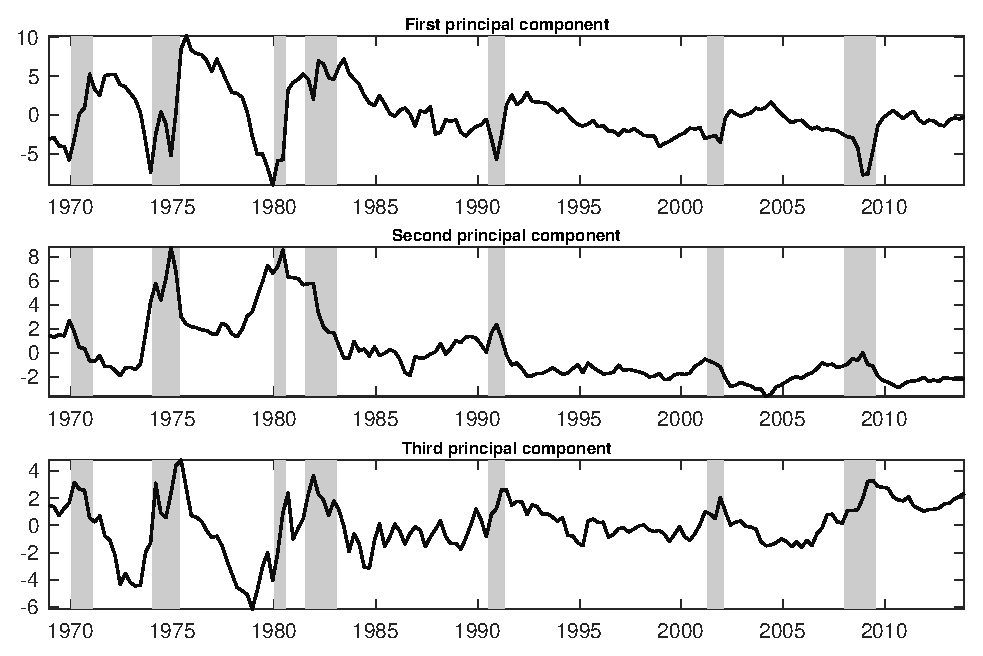
\includegraphics[scale=1]{figures/e_principal_components.eps}
    \label{Fig:e_principal_components}
\end{figure}


% TIME SERIES DYNAMICS OF THE ME FACTORS
\clearpage
\begin{figure}[htbp]
    \caption{
        \textbf{Time series dynamics of the ME$_{t}$ factor.} \newline
        This figure illustrates the relation between expected business conditions $\left(\text{ME}_{t}\right)$ and the real economy as measured by the Chicago National Activity Index (CFNAI$_{t}$) and National Bureau of Economic Research (NBER) defined recession periods in gray shading over the sample period 1968:Q4-2014:Q4. ME$_{t}$ and CFNAI$_{t}$ are plotted in standardized units for convenience. 
    }
    \centering
    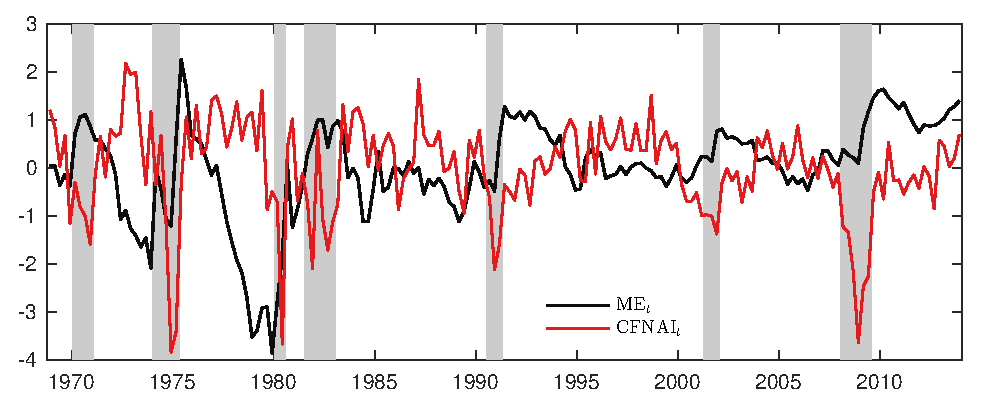
\includegraphics[scale=1]{figures/e_me_cfnai.eps}
    \label{Fig:e_me_cfnai}
\end{figure}

% CUMULATIVE DIFFERENCES IN SQUARED FORECAST ERRORS
\clearpage
\begin{figure}[htbp]
    \caption{
        \textbf{Differences in cumulative squared prediction errors.} \newline
        This figure illustrates the relative forecasting performance by plotting the difference in cumulative squared prediction errors from (\ref{eq:e_dcsfe}) between the candidate forecasting model and the expectations hypothesis (EH) model  over the out-of-sample evaluation period, which covers the period from 1990:Q1 to 2014:Q4. National Bureau of Economic Research (NBER) recession periods are marked in gray shading.
    }
    \centering
    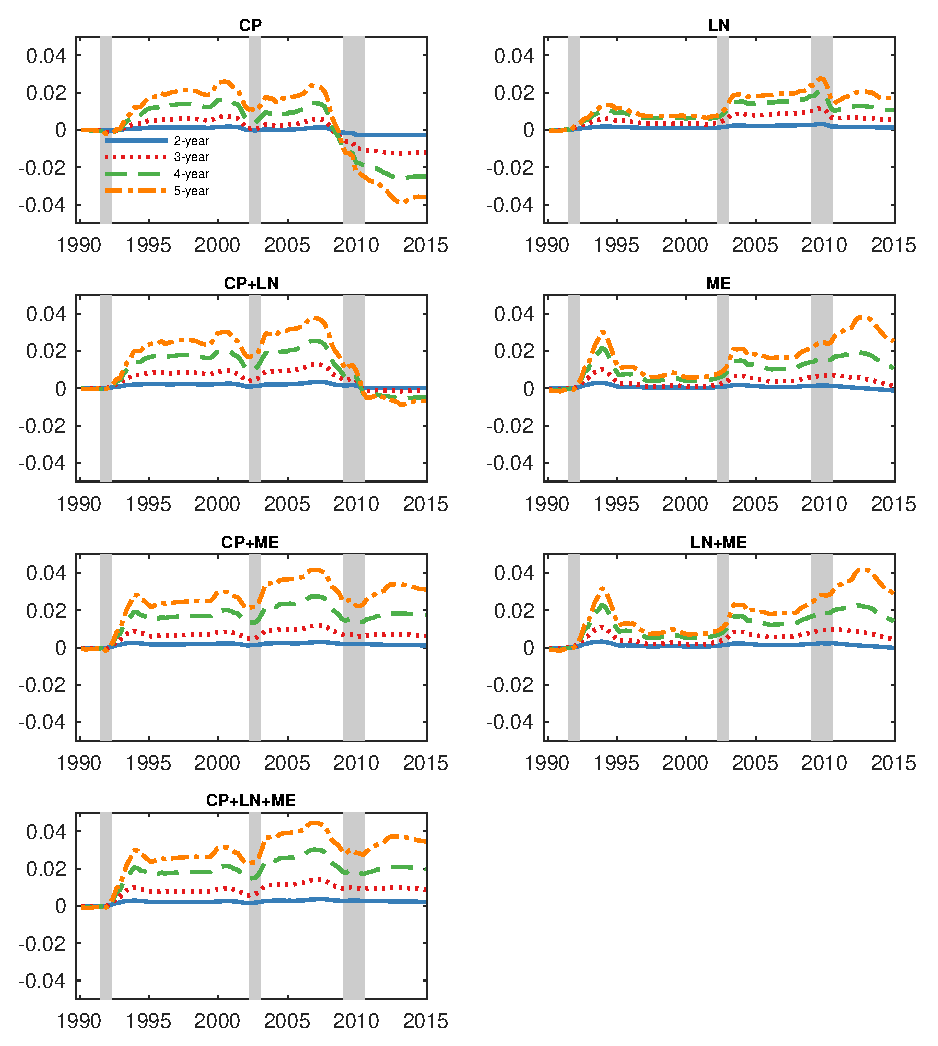
\includegraphics[scale=1]{figures/e_dcsfe.eps}
    \label{Fig:e_dcsfe}
\end{figure}

% CUMULATIVE DIFFERENCES IN UTILITY GAINS
\clearpage
\begin{figure}[htbp]
    \caption{
        \textbf{Differences in cumulative realized utility.} \newline
        This figure illustrates the relative portfolio performance by plotting the difference in cumulative realized utility from (\ref{eq:e_average_utility}) between the candidate forecasting model and the expectations hypothesis (EH) model  over the out-of-sample evaluation period, which covers the period from 1990:Q1 to 2014:Q4. National Bureau of Economic Research (NBER) recession periods are marked in gray shading.
    }
    \centering
    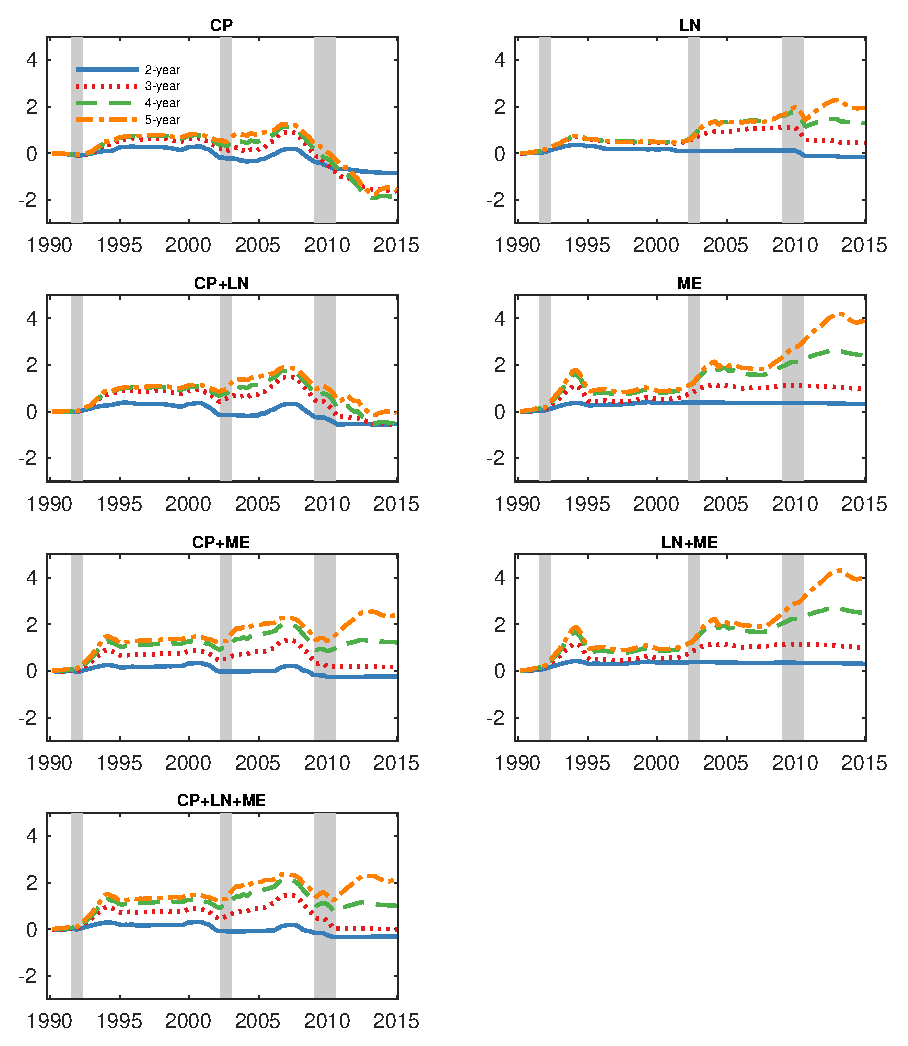
\includegraphics[scale=1]{figures/e_dcutil.eps}
    \label{Fig:e_dcutil}
\end{figure}

%----------------------------------------------------------------------------------------------------------------------
% TABLES
%----------------------------------------------------------------------------------------------------------------------

% SUMMARY STATISTICS FOR SPF VARIABLES
\clearpage
\begin{table}[htbp]
    \footnotesize
    \caption{
        \textbf{Descriptive statistics: Survey variables.} \newline
        This table reports descriptive statistics for the median expected growth rates for the macroeconomic fundamentals collected from the Survey of Professional Forecasters (SPF). The variables include: 1) GDP $\left(\text{gdp}_{t}^{\mathbb{E}}\right)$, 2) the GDP price index $\left(\text{inf}_{t}^{\mathbb{E}}\right)$, 3) the unemployment rate $\left(\text{unemp}_{t}^{\mathbb{E}}\right)$, 4) corporate profits after tax $\left(\text{cprof}_{t}^{\mathbb{E}}\right)$, 5) industrial production $\left(\text{ip}_{t}^{\mathbb{E}}\right)$, and 6) housing starts $\left(\text{hous}_{t}^{\mathbb{E}}\right)$. We report means, standard deviations, skewness, and kurtosis for each fundamental and forecast horizon. The last three rows in each panel reports the loadings from the principal component estimation. The sample covers the period from 1968:Q4 to 2014:Q4.
    }
    \centering
    \begin{tabularx}{\textwidth}{ZYYYYYYYYYYY}
        \toprule
         & gdp$_{t}^{\mathbb{E}}$ & inf$_{t}^{\mathbb{E}}$ & cprof$_{t}^{\mathbb{E}}$ & unemp$_{t}^{\mathbb{E}}$ & ip$_{t}^{\mathbb{E}}$ & hous$_{t}^{\mathbb{E}}$ \\\midrule
 & \multicolumn{6}{c}{Panel A: One quarter ahead} \\\cmidrule{2-7}
Mean & 1.53 & 0.88 & 1.42 & 0.51 & 0.77 & 0.23 \\
Std & 0.57 & 0.50 & 2.11 & 2.74 & 0.79 & 5.67 \\
Skewness & 0.63 & 1.18 & -0.70 & 1.01 & -0.67 & -0.05 \\
Kurtosis & 3.18 & 3.55 & 5.46 & 3.31 & 5.79 & 4.42 \\
Load $\mathcal{P}_{1,t}^{\mathbb{E}}$ & 0.22 & 0.07 & 0.24 & -0.20 & 0.24 & 0.14 \\
Load $\mathcal{P}_{2,t}^{\mathbb{E}}$ & 0.18 & 0.36 & -0.16 & 0.20 & -0.15 & 0.06 \\
Load $\mathcal{P}_{3,t}^{\mathbb{E}}$ & -0.21 & -0.10 & -0.03 & 0.16 & -0.10 & 0.43 \\\cmidrule{2-7}
 & \multicolumn{6}{c}{Panel B: Two quarter ahead} \\\cmidrule{2-7}
Mean & 3.13 & 1.77 & 3.19 & 0.52 & 1.66 & 1.67 \\
Std & 1.11 & 0.97 & 3.50 & 4.78 & 1.32 & 10.12 \\
Skewness & 0.73 & 1.15 & -0.37 & 1.10 & -0.66 & 0.20 \\
Kurtosis & 2.95 & 3.49 & 4.95 & 3.74 & 5.87 & 3.79 \\
Load $\mathcal{P}_{1,t}^{\mathbb{E}}$ & 0.22 & 0.08 & 0.26 & -0.23 & 0.26 & 0.12 \\
Load $\mathcal{P}_{2,t}^{\mathbb{E}}$ & 0.21 & 0.36 & -0.12 & 0.19 & -0.12 & 0.11 \\
Load $\mathcal{P}_{3,t}^{\mathbb{E}}$ & -0.17 & -0.10 & 0.04 & 0.09 & -0.03 & 0.45 \\\cmidrule{2-7}
 & \multicolumn{6}{c}{Panel C: Three quarter ahead} \\\cmidrule{2-7}
Mean & 4.76 & 2.65 & 5.19 & -0.08 & 2.63 & 3.73 \\
Std & 1.62 & 1.42 & 4.45 & 5.81 & 1.64 & 14.32 \\
Skewness & 0.78 & 1.09 & 0.23 & 0.89 & -0.06 & 0.48 \\
Kurtosis & 2.83 & 3.36 & 4.02 & 3.29 & 4.38 & 3.69 \\
Load $\mathcal{P}_{1,t}^{\mathbb{E}}$ & 0.21 & 0.08 & 0.26 & -0.24 & 0.27 & 0.09 \\
Load $\mathcal{P}_{2,t}^{\mathbb{E}}$ & 0.23 & 0.36 & -0.07 & 0.17 & -0.08 & 0.16 \\
Load $\mathcal{P}_{3,t}^{\mathbb{E}}$ & -0.14 & -0.11 & 0.09 & 0.02 & 0.01 & 0.45 \\\cmidrule{2-7}
 & \multicolumn{6}{c}{Panel D: Four quarter ahead} \\\cmidrule{2-7}
Mean & 6.44 & 3.54 & 7.06 & -0.97 & 3.61 & 5.79 \\
Std & 2.15 & 1.86 & 5.09 & 6.55 & 1.91 & 17.78 \\
Skewness & 0.83 & 1.08 & 0.72 & 0.64 & 0.48 & 0.56 \\
Kurtosis & 2.78 & 3.34 & 3.56 & 2.79 & 3.88 & 3.60 \\
Load $\mathcal{P}_{1,t}^{\mathbb{E}}$ & 0.20 & 0.09 & 0.25 & -0.25 & 0.28 & 0.06 \\
Load $\mathcal{P}_{2,t}^{\mathbb{E}}$ & 0.26 & 0.35 & -0.01 & 0.14 & -0.04 & 0.19 \\
Load $\mathcal{P}_{3,t}^{\mathbb{E}}$ & -0.12 & -0.11 & 0.13 & -0.03 & 0.04 & 0.43 \\


        \bottomrule
        \label{Tab:e_sumstat_survey_variables}
    \end{tabularx}
\end{table}


% ESTIMATING THE MACRO-EXPECTATIONS FACTOR
\clearpage
\begin{table}[htbp]
    \footnotesize
    \caption{
        \textbf{Estimating the macroeconomic expectations factor.} \newline
        This table reports slope estimates from regressing one-year ahead bond risk premia upon the first three principal components ($\mathcal{P}_{1,t}^{\mathbb{E}}$,$\mathcal{P}_{2,t}^{\mathbb{E}}$,$\mathcal{P}_{3,t}^{\mathbb{E}}$) of the Survey of Professional Forecasters (SPF) forecasts and expected business conditions $\left(\text{ME}_{t}\right)$ in rows (a) and (b), respectively. Although not reported, all regressions contain an intercept. \cite{HansenHodrick1980} t-statistics implemented with four lags are presented in parentheses. Adj. R$^{2}\left(\%\right)$ denotes the full sample adjusted coefficient of determination in percentage. The sample period starts in 1968:Q4 and ends in 2014:Q4.
    }
    \centering
    \begin{tabularx}{\textwidth}{lYYYYYY}
        \toprule
         & $\mathcal{P}_{1,t}^{\mathbb{E}}$ & $\mathcal{P}_{2,t}^{\mathbb{E}}$ & $\mathcal{P}_{3,t}^{\mathbb{E}}$ & ME$_{t}$ & adj R$^{2}\left(\%\right)$ \\\midrule
 & \multicolumn{5}{c}{Panel A: Two-year bond} \\\cmidrule{2-6}
(a) & 0.08 & -0.10 & 0.38 &  & 18.87 \\
 & (2.03) & (-1.18) & (3.32) &  &  \\
(b) &  &  &  & 0.46 & 18.86 \\
 &  &  &  & (4.56) &  \\\cmidrule{2-6}
 & \multicolumn{5}{c}{Panel B: Three-year bond} \\\cmidrule{2-6}
(a) & 0.13 & -0.24 & 0.67 &  & 19.22 \\
 & (1.79) & (-1.58) & (3.49) &  &  \\
(b) &  &  &  & 0.86 & 19.85 \\
 &  &  &  & (4.71) &  \\\cmidrule{2-6}
 & \multicolumn{5}{c}{Panel C: Four-year bond} \\\cmidrule{2-6}
(a) & 0.20 & -0.43 & 0.83 &  & 18.99 \\
 & (2.03) & (-2.10) & (3.38) &  &  \\
(b) &  &  &  & 1.20 & 19.84 \\
 &  &  &  & (4.80) &  \\\cmidrule{2-6}
 & \multicolumn{5}{c}{Panel D: Five-year bond} \\\cmidrule{2-6}
(a) & 0.24 & -0.56 & 0.99 &  & 19.56 \\
 & (2.00) & (-2.42) & (3.57) &  &  \\
(b) &  &  &  & 1.47 & 20.29 \\
 &  &  &  & (4.90) &  \\


        \bottomrule
        \label{Tab:e_me_estimation}
    \end{tabularx}
\end{table}


% SUMMARY STATISTICS
\clearpage
\begin{table}[htbp]
    \footnotesize
    \caption{
        \textbf{Descriptive statistics: Bond risk premia and forecasting factors.} \newline
        This table reports descriptive statistics for excess bond returns $rx_{t+4}^{\left(n\right)}$, $n=2,\ldots,5$ and predictor variables used in the empirical analyses (Panel A) and their contemporaneous correlations (Panel B). CP$_{t}$ is the forward rate-based factor from \cite{CochranePiazzesi2005}, LN$_{t}$ is the macro-based factor from \cite{LudvigsonNg2009}, and ME$_{t}$ represents our proxy for expected business conditions described in Section \ref{Sec:e_measuring_ebc}. For each variable, we report means, standard deviations, skewness, and kurtosis as well as first- and second-order autocorrelations. In addition, we report Sharpe ratios (SR) for each of the Treasury bonds. The sample covers the period from 1968:Q4 to 2014:Q4.
    }
    \centering
    \begin{tabularx}{\linewidth}{ZYYYYYYYY}
        \toprule
         & $rx^{\left(2\right)}_{t+4}$ & $rx^{\left(3\right)}_{t+4}$ & $rx^{\left(4\right)}_{t+4}$ & $rx^{\left(5\right)}_{t+4}$ & CP$_{t}$ & LN$_{t}$ & ME$_{t}$ \\\midrule
 & \multicolumn{7}{c}{Panel A: Descriptive statistics} \\\cmidrule{2-8}
Mean & 0.60 & 1.06 & 1.48 & 1.63 & 1.19 & 1.19 & 1.19 \\
Std & 1.79 & 3.27 & 4.54 & 5.52 & 1.54 & 1.56 & 1.70 \\
Skewness & -0.24 & -0.29 & -0.28 & -0.20 & -0.10 & -0.72 & -1.22 \\
Kurtosis & 3.73 & 3.72 & 3.76 & 3.44 & 3.80 & 5.79 & 5.48 \\
AC(1) & 0.75 & 0.74 & 0.75 & 0.74 & 0.68 & 0.57 & 0.89 \\
AC(4) & 0.20 & 0.15 & 0.14 & 0.10 & 0.42 & 0.13 & 0.62\\
SR & 0.34 & 0.33 & 0.33 & 0.30 & - & - & - \\\cmidrule{2-8}
 & \multicolumn{7}{c}{Panel B: Correlation matrix} \\\cmidrule{2-8}
$rx^{\left(2\right)}_{t+4}$ & 1.00 &  &  &  &  &  &  \\
$rx^{\left(3\right)}_{t+4}$ & 0.98 & 1.00 &  &  &  &  &  \\
$rx^{\left(4\right)}_{t+4}$ & 0.96 & 0.99 & 1.00 &  &  &  &  \\
$rx^{\left(5\right)}_{t+4}$ & 0.93 & 0.97 & 0.99 & 1.00 &  &  &  \\
CP$_{t}$ & 0.37 & 0.40 & 0.43 & 0.40 & 1.00 &  &  \\
LN$_{t}$ & 0.41 & 0.43 & 0.42 & 0.40 & 0.11 & 1.00 &  \\
ME$_{t}$ & 0.44 & 0.45 & 0.45 & 0.46 & 0.42 & 0.33 & 1.00 \\


        \bottomrule
        \label{Table:e_sumstat_brp_factor}
    \end{tabularx}
\end{table}

% JOSLIN-PRIEBSCH-SINGLETON MACRO-SPANNING CONDITION
\clearpage
\begin{table}[htbp]
    \footnotesize
    \caption{
        \textbf{Macro-spanning condition for expected business conditions.} \newline
        This table reports slope estimates from the \cite{JoslinPriebschSingleton2014} macro-spanning condition in (\ref{eq:e_macro_spanning_condition}). Although not reported, all regressions contain an intercept. $\mathcal{P}_{1,t}^{\mathbb{E}}$, $\mathcal{P}_{2,t}^{\mathbb{E}}$, and $\mathcal{P}_{3,t}^{\mathbb{E}}$ denote the first three principal components estimated from survey forecasts and level$_{t}$, slope$_{t}$, curv$_{t}$, $\mathcal{Y}_{4,t}$, and $\mathcal{Y}_{5,t}$ are the principal components of the yield covariance matrix. \cite{NeweyWest1987} t-statistics implemented with six lags are presented in parentheses. Adj. R$^{2}\left(\%\right)$ denotes the full sample adjusted coefficient of determination in percentage. The sample period starts in 1968:Q4 and ends in 2014:Q4.
    }
    \centering
    \begin{tabularx}{\textwidth}{ZYYYYYYc}
        \toprule
         & Variable & level$_{t}$ & slope$_{t}$ & curv$_{t}$ & $\mathcal{Y}_{4,t}$ & $\mathcal{Y}_{5,t}$ & adj R$^{2}\left(\%\right)$ \\\midrule
(a) & $\mathcal{P}_{1,t}^{\mathbb{E}}$ & 0.12 & 2.51 & -0.55 &  &  & 28.15 \\
 &  & (1.82) & (4.35) & (-0.16) &  &  &  \\
(b) &  & 0.12 & 2.51 & -0.55 & -0.51 & 4.28 & 27.87 \\
 &  & (1.88) & (4.46) & (-0.16) & (-0.10) & (0.77) &  \\\cmidrule{2-8}
(a) & $\mathcal{P}_{2,t}^{\mathbb{E}}$ & 0.25 & -1.16 & 4.97 &  &  & 60.67 \\
 &  & (8.36) & (-3.46) & (2.75) &  &  &  \\
(b) &  & 0.26 & -1.16 & 4.97 & 0.27 & 7.42 & 62.97 \\
 &  & (8.66) & (-3.55) & (3.07) & (0.09) & (3.54) &  \\\cmidrule{2-8}
(a) & $\mathcal{P}_{3,t}^{\mathbb{E}}$ & -0.07 & 0.54 & 2.22 &  &  & 10.57 \\
 &  & (-1.42) & (1.53) & (1.72) &  &  &  \\
(b) &  & -0.07 & 0.54 & 2.24 & 6.17 & 5.31 & 17.75 \\
 &  & (-1.84) & (1.94) & (1.78) & (2.52) & (1.98) &  \\\cmidrule{2-8}
(a) & ME$_{t}$ & -0.12 & 1.19 & -0.14 &  &  & 42.17 \\
 &  & (-2.72) & (3.46) & (-0.20) &  &  &  \\
(b) &  & -0.12 & 1.19 & -0.13 & 4.27 & 2.05 & 45.23 \\
 &  & (-3.20) & (3.93) & (-0.14) & (1.68) & (1.13) &  \\


        \bottomrule
        \label{Tab:e_spanning_restriction}
    \end{tabularx}
\end{table}


% IN-SAMPLE RESULTS
\clearpage
\begin{table}[htbp]
    \scriptsize
    \caption{
        \textbf{In-sample results.} \newline
        This table reports slope estimates from regressing one-year ahead bond risk premia upon various combinations of predictors. CP$_{t}$ is the forward rate-based factor from \cite{CochranePiazzesi2005}, LN$_{t}$ is the macro-based factor from \cite{LudvigsonNg2009}, and ME$_{t}$ represents our proxy for expected business conditions described in Section \ref{Sec:e_measuring_ebc}. Although not reported, all regressions contain an intercept. \cite{HansenHodrick1980} t-statistics implemented with four lags are presented in parentheses. Adj. R$^{2}\left(\%\right)$ denotes the full sample adjusted coefficient of determination in percentage. The sample period starts in 1968:Q4 and ends in 2014:Q4.
    }
    \centering
    \begin{tabularx}{\textwidth}{lYYYYYYY}
        \toprule
         & CP$_{t}$ & LN$_{t}$ & ME$_{t}$ & adj R$^{2}\left(\%\right)$ \\\midrule
 & \multicolumn{4}{c}{Panel A: Two-year bond} \\\cmidrule{2-5}
(a) & 0.43 &  &  & 13.17 \\
 & (3.44) &  &  &  \\
(b) & 0.26 &  & 0.36 & 22.55 \\
 & (1.63) &  & (2.80) &  \\
(c) &  & 0.47 &  & 16.47 \\
 &  & (3.58) &  &  \\
(d) &  & 0.34 & 0.36 & 26.52 \\
 &  & (3.98) & (3.78) &  \\
(e) & 0.38 & 0.43 &  & 26.82 \\
 & (2.94) & (3.95) &  &  \\
(f) & 0.27 & 0.35 & 0.25 & 30.72 \\
 & (1.65) & (4.69) & (2.06) &  \\\cmidrule{2-5}
 & \multicolumn{4}{c}{Panel B: Three-year bond} \\\cmidrule{2-5}
(a) & 0.84 &  &  & 15.16 \\
 & (3.40) &  &  &  \\
(b) & 0.53 &  & 0.66 & 24.56 \\
 & (1.90) &  & (3.06) &  \\
(c) &  & 0.90 &  & 18.06 \\
 &  & (4.21) &  &  \\
(d) &  & 0.66 & 0.66 & 28.46 \\
 &  & (4.74) & (3.57) &  \\
(e) & 0.75 & 0.82 &  & 30.07 \\
 & (3.08) & (5.00) &  &  \\
(f) & 0.56 & 0.68 & 0.45 & 33.77 \\
 & (1.95) & (6.03) & (2.09) &  \\\cmidrule{2-5}
 & \multicolumn{4}{c}{Panel C: Four-year bond} \\\cmidrule{2-5}
(a) & 1.28 &  &  & 18.39 \\
 & (3.59) &  &  &  \\
(b) & 0.87 &  & 0.87 & 26.69 \\
 & (2.13) &  & (2.95) &  \\
(c) &  & 1.22 &  & 17.10 \\
 &  & (4.25) &  &  \\
(d) &  & 0.89 & 0.93 & 27.74 \\
 &  & (4.53) & (3.62) &  \\
(e) & 1.16 & 1.10 &  & 32.12 \\
 & (3.24) & (5.15) &  &  \\
(f) & 0.91 & 0.92 & 0.58 & 35.28 \\
 & (2.15) & (5.79) & (1.92) &  \\\cmidrule{2-5}
 & \multicolumn{4}{c}{Panel D: Five-year bond} \\\cmidrule{2-5}
(a) & 1.45 &  &  & 15.93 \\
 & (3.16) &  &  &  \\
(b) & 0.93 &  & 1.12 & 25.38 \\
 & (1.78) &  & (3.01) &  \\
(c) &  & 1.40 &  & 15.25 \\
 &  & (4.48) &  &  \\
(d) &  & 0.98 & 1.18 & 26.78 \\
 &  & (4.56) & (3.67) &  \\
(e) & 1.31 & 1.26 &  & 28.21 \\
 & (2.85) & (5.18) &  &  \\
(f) & 0.97 & 1.01 & 0.80 & 32.41 \\
 & (1.79) & (5.33) & (2.04) &  \\


        \bottomrule
        \label{Tab:e_insample_results}
    \end{tabularx}
\end{table}

% OUT-OF-SAMPLE RESULTS
\clearpage
\begin{table}[htbp]
    \footnotesize
    \caption{
        \textbf{Out-sample-results.} \newline
        This table reports the out-of-sample results from forecasting one-year ahead bond risk premia using various combinations of predictors. CP$_{t}$ is the forward rate-based factor from \cite{CochranePiazzesi2005}, LN$_{t}$ is the macro-based factor from \cite{LudvigsonNg2009}, and ME$_{t}$ represents our proxy for expected business conditions described in Section \ref{Sec:e_measuring_ebc}. Panel A reports the \cite{CampbellThompson2008} R$^{2}_{oos}$ statistic from (\ref{eq:e_r2oos}) relative to the expectations hypothesis (EH) benchmark accompanied by p-values from \cite{ClarkWest2007} tests of equal predictive ability in square brackets. Panel B reports annualized percentage utility gain, $\Delta\left(\%\right)$, relative to the EH model accompanied by p-valued from \cite{DieboldMariano1995} tests of equal utilities in square brackets. Finally, Panel C reports annualized \cite{GoetzmannIngersollSpiegelWelch} manipulation-proof performance measures, $\Theta\left(\%\right)$. The out-of-sample evaluation period starts in 1990:Q1 and ends in 2014:Q4.
    }
    \centering
    \begin{tabularx}{\textwidth}{lYYYYYYY}
        \toprule
        n & CP & LN & CP+LN & ME & CP+ME & LN+ME & CP+LN+ME \\\midrule
 & \multicolumn{7}{c}{Panel A: R$^{2}_{\text{oos}}$} \\\cmidrule{2-8}
2 & -16.26 & 7.57 & 0.80 & -7.17 & 6.53 & -1.13 & 12.31 \\
 & [0.17] & [0.01] & [0.02] & [0.07] & [0.04] & [0.05] & [0.03] \\
3 & -20.10 & 9.08 & -2.05 & 2.08 & 10.15 & 6.99 & 14.54 \\
 & [0.24] & [0.01] & [0.04] & [0.03] & [0.03] & [0.02] & [0.02] \\
4 & -20.27 & 8.77 & -3.98 & 8.77 & 14.06 & 11.51 & 16.09 \\
 & [0.20] & [0.01] & [0.05] & [0.02] & [0.02] & [0.02] & [0.02] \\
5 & -18.62 & 8.82 & -3.54 & 13.08 & 16.12 & 15.05 & 17.86 \\
 & [0.28] & [0.01] & [0.07] & [0.01] & [0.02] & [0.01] & [0.02] \\\cmidrule{2-8}
 & \multicolumn{7}{c}{Panel B: $\Delta\left(\%\right)$} \\\cmidrule{2-8}
2 & -0.84 & -0.15 & -0.54 & 0.32 & -0.23 & 0.31 & -0.31 \\
 & [0.97] & [0.75] & [0.88] & [0.01] & [0.75] & [0.02] & [0.82] \\
3 & -1.64 & 0.43 & -0.57 & 0.96 & 0.16 & 0.99 & -0.00 \\
 & [0.98] & [0.17] & [0.77] & [0.04] & [0.40] & [0.04] & [0.50] \\
4 & -1.95 & 1.28 & -0.56 & 2.39 & 1.21 & 2.46 & 0.99 \\
 & [0.99] & [0.02] & [0.74] & [0.00] & [0.06] & [0.00] & [0.11] \\
5 & -1.57 & 1.93 & -0.09 & 3.85 & 2.38 & 3.95 & 2.10 \\
 & [0.97] & [0.00] & [0.53] & [0.00] & [0.00] & [0.00] & [0.01] \\\cmidrule{2-8}
 & \multicolumn{7}{c}{Panel C: $\Theta\left(\%\right)$} \\\cmidrule{2-8}
2 & -0.90 & -0.03 & -0.61 & 0.47 & -0.27 & 0.46 & -0.34 \\
3 & -1.40 & 0.76 & -0.37 & 1.34 & 0.27 & 1.39 & 0.18 \\
4 & -1.42 & 1.56 & -0.14 & 2.86 & 1.41 & 2.97 & 1.30 \\
5 & -1.06 & 2.06 & 0.40 & 4.01 & 2.51 & 4.19 & 2.39 \\


        \bottomrule
        \label{Tab:e_out_of_sample_results}
    \end{tabularx}
\end{table}

% MODEL COMPARISONS
\clearpage
\begin{table}[htbp]
    \footnotesize
    \caption{
        \textbf{Model Comparisons.} \newline
        This table reports the out-of-sample results from forecasting one-year ahead bond risk premia using nested models with and without expected business conditions $\left(\text{ME}_{t}\right)$. R$^{2}_{\text{oos}}$ is the out-of-sample R$^{2}$ suggested in \cite{CampbellThompson2008}. For each R$^{2}_{\text{oos}}$, we report p-values from the \cite{ClarkWest2007} test of equal predictive ability in square brackets. $\Delta\left(\%\right)$ denotes the annualized percentage utility gain between the model including expected business conditions and the nested benchmark omitting expected business conditions. $\Theta\left(\%\right)$ is the annualized manipulation-proof measure from \cite{GoetzmannIngersollSpiegelWelch}. For each $\Delta\left(\%\right)$, we report p-values from the \cite{DieboldMariano1995} test in square brackets. The out-of-sample evaluation period starts in 1990:Q1 and ends in 2014:Q4.
    }
    \centering
    \begin{tabularx}{\textwidth}{lYYYYYYYYYY}
        \toprule
         & R$^{2}_{\text{oos}}$ & p-val & $\Delta$(\%) & p-val & $\Theta$(\%) \\\midrule
 & \multicolumn{5}{c}{Panel A: Two-year bond} \\\cmidrule{2-6}
CP+ME vs. CP & 19.60 & [0.00] & 0.61 & [0.03] & 0.63  \\
LN+ME vs. LN & -9.41 & [0.16] & 0.46 & [0.01] & 0.49 \\
CP+LN+ME vs. CP+LN & 11.60 & [0.02] & 0.23 & [0.19] & 0.27 \\\cmidrule{2-6}
 & \multicolumn{5}{c}{Panel B: Three-year bond} \\\cmidrule{2-6}
CP+ME vs. CP & 25.19 & [0.00] & 1.80 & [0.00] & 1.67 \\
LN+ME vs. LN & -2.30 & [0.11] & 0.55 & [0.13] & 0.62 \\
CP+LN+ME vs. CP+LN & 16.25 & [0.01] & 0.57 & [0.07] & 0.56 \\\cmidrule{2-6}
 & \multicolumn{5}{c}{Panel C: Four-year bond} \\\cmidrule{2-6}
CP+ME vs. CP & 28.54 & [0.00] & 3.16 & [0.00] & 2.83 \\
LN+ME vs. LN & 3.00 & [0.07] & 1.18 & [0.05] & 1.41 \\
CP+LN+ME vs. CP+LN & 19.30 & [0.00] & 1.56 & [0.00] & 1.44 \\\cmidrule{2-6}
 & \multicolumn{5}{c}{Panel D: Five-year bond} \\\cmidrule{2-6}
CP+ME vs. CP & 29.28 & [0.00] & 3.95 & [0.00] & 3.58 \\
LN+ME vs. LN & 6.83 & [0.05] & 2.02 & [0.01] & 2.13 \\
CP+LN+ME vs. CP+LN & 20.67 & [0.00] & 2.19 & [0.00] & 2.00 \\


        \bottomrule
        \label{Tab:e_out_of_sample_model_comparison}
    \end{tabularx}
\end{table}

 
% OUT-OF-SAMPLE FORECAST COMBINATION RESULTS
\clearpage
\begin{table}[htbp]
    \footnotesize
    \caption{
        \textbf{Forecast combination.} \newline
        This table reports the out-of-sample results from forecasting one-year ahead bond risk premia using combinations of forecasts. Panel A presents the results from combining forecasts from the three CP$_{t}$ and LN$_{t}$ models and Panel B presents the results from combining forecasts for all seven model. R$^{2}_{\text{oos}}$ is the out-of-sample R$^{2}$ suggested in \cite{CampbellThompson2008}. For each R$^{2}_{\text{oos}}$, we report p-values from the \cite{ClarkWest2007} test of equal predictive ability in square brackets. $\Delta\left(\%\right)$ denotes the annualized percentage utility gain between the model including expected business conditions and the nested benchmark omitting expected business conditions. $\Theta\left(\%\right)$ is the annualized manipulation-proof measure from \cite{GoetzmannIngersollSpiegelWelch}. For each $\Delta\left(\%\right)$, we report p-values from the \cite{DieboldMariano1995} test in square brackets. The out-of-sample evaluation period starts in 1990:Q1 and ends in 2014:Q4.
    }
    \centering
    \begin{tabularx}{\textwidth}{lYYYYYYYYYYYYYY}
        \toprule
        n & R$^{2}_{\text{oos}}$ & p-val & $\Delta$(\%) & p-val & $\Theta$(\%) \\\midrule
 & \multicolumn{5}{c}{Panel A: Forecast combination using CP$_{t}$ and LN$_{t}$ models} \\\cmidrule{2-6}
2 & 8.00 & [0.02] & -0.41 & [0.85] & -0.46 \\
3 & 5.98 & [0.04] & -0.50 & [0.76] & -0.39 \\
4 & 5.05 & [0.04] & -0.50 & [0.74] & -0.22 \\
5 & 3.85 & [0.06] & -0.07 & [0.53] & 0.21 \\\cmidrule{2-6}
 & \multicolumn{5}{c}{Panel B: Forecast combination using all models} \\\cmidrule{2-6}
2 & 15.81 & [0.02] & 0.13 & [0.28] & 0.16 \\
3 & 17.71 & [0.02] & 0.42 & [0.23] & 0.61 \\
4 & 19.60 & [0.01] & 1.22 & [0.04] & 1.39 \\
5 & 19.41 & [0.01] & 2.11 & [0.00] & 2.17 \\


        \bottomrule
        \label{Tab:e_forecast_combination}
    \end{tabularx}
\end{table}


% % CORRELATION MEASURES OF FORECASTING PERFORMANCE
\clearpage
\begin{table}[htbp]
    \footnotesize
    \caption{
        \textbf{Forecast performance, expected returns, and economic variables.} \newline
        This table reports contemporaneous correlations between relative forecast and portfolio performance and the real economy as measured by the Chicago Fed National Activity Index $\left(\text{CFNAI}_{t}\right)$ in Panels A and B. Relative forecast performance is defined as the difference in cumulative squared prediction error $\left(\text{DCSPE}_{t}\right)$ from (\ref{eq:e_dcsfe}) and portfolio performance is the cumulative difference in realized utilities $\left(\text{DCRU}_{t}\right)$ from (\ref{eq:e_average_utility}). Panels C and D report contemporaneous correlations between expected bond risk premia and the CFNAI$_{t}$ and macroeconomic uncertainty $\left(\mathbb{U}_{t}^{\text{Macro}}\right)$, respectively. Macro uncertainty is the uncertainty index constructed in \cite{JuradoLudvgisonNg2015}. The out-of-sample evaluation period starts in 1990:Q1 and ends in 2014:Q4.
    }
    \centering
    \begin{tabularx}{\textwidth}{lYYYYcYYYY}
        \toprule
         & 2-year & 3-year & 4-year & 5-year &  & 2-year & 3-year & 4-year & 5-year \\\midrule
 & \multicolumn{4}{c}{Panel A: $\rho\left(\text{DCSPE}_{t},\text{CFNAI}_{t}\right)$} &  & \multicolumn{4}{c}{Panel B: $\rho\left(\text{DCRU}_{t},\text{CFNAI}_{t}\right)$}  \\\cmidrule{2-5}\cmidrule{7-10}
CP & 0.53 & 0.49 & 0.47 & 0.44 &  & 0.48 & 0.37 & 0.30 & 0.26 \\
LN & -0.25 & -0.25 & -0.22 & -0.25 &  & 0.24 & -0.14 & -0.27 & -0.27 \\
CP+LN & 0.42 & 0.42 & 0.44 & 0.41 &  & 0.50 & 0.38 & 0.29 & 0.23 \\
ME & -0.31 & -0.42 & -0.32 & -0.26 &  & 0.02 & -0.28 & -0.27 & -0.24 \\
CP+ME & 0.16 & 0.24 & 0.29 & 0.23 &  & 0.54 & 0.45 & 0.31 & 0.14 \\
LN+ME & -0.41 & -0.42 & -0.32 & -0.27 &  & 0.04 & -0.28 & -0.27 & -0.25 \\
CP+LN+ME & 0.03 & 0.12 & 0.22 & 0.17 &  & 0.49 & 0.41 & 0.29 & 0.16 \\
FC1 & 0.25 & 0.30 & 0.33 & 0.32 &  & 0.50 & 0.38 & 0.31 & 0.24 \\
FC2 & -0.08 & -0.03 & 0.02 & 0.02 &  & 0.30 & 0.27 & 0.18 & 0.07 \\\cmidrule{2-5}\cmidrule{7-10}
 & \multicolumn{4}{c}{Panel C: $\rho\left(\mathbb{E}_{t}rx_{t+4}^{\left(n\right)},\text{CFNAI}_{t}\right)$} &  & \multicolumn{4}{c}{Panel D: $\rho\left(\mathbb{E}_{t}rx_{t+4}^{\left(n\right)},\mathbb{U}_{t}^{\text{Macro}}\right)$}  \\\cmidrule{2-5}\cmidrule{7-10}
CP & 0.03 & 0.02 & 0.03 & 0.02 &  & -0.24 & -0.23 & -0.24 & -0.23 \\
LN & -0.09 & -0.09 & -0.07 & -0.07 &  & -0.14 & -0.13 & -0.13 & -0.11 \\
CP+LN & -0.02 & -0.02 & 0.01 & 0.00 &  & -0.29 & -0.28 & -0.30 & -0.28 \\
ME & -0.43 & -0.43 & -0.42 & -0.42 &  & 0.18 & 0.20 & 0.20 & 0.20 \\
CP+ME & -0.29 & -0.27 & -0.23 & -0.26 &  & 0.02 & 0.02 & -0.03 & 0.01 \\
LN+ME & -0.37 & -0.37 & -0.34 & -0.36 &  & 0.06 & 0.07 & 0.06 & 0.10 \\
CP+LN+ME & -0.23 & -0.21 & -0.15 & -0.19 &  & -0.10 & -0.11 & -0.16 & -0.10 \\
FC1 & -0.03 & -0.03 & -0.00 & -0.01 &  & -0.28 & -0.27 & -0.28 & -0.26 \\
FC2 & -0.24 & -0.23 & -0.20 & -0.22 &  & -0.09 & -0.09 & -0.11 & -0.07 \\


        \bottomrule
        \label{Tab:e_links_to_the_real_economy}
    \end{tabularx}
\end{table}

% IN-SAMPLE RESULTS FOR GSW BOND DATA
\clearpage
\begin{table}[htbp]
    \caption{
        \textbf{In-sample results for quarterly bond risk premia.} \newline
        This table reports slope estimates from regressing one-quarter ahead bond risk premia upon various combinations of predictors. CP$_{t}^{\text{GSW}}$ is the forward rate-based factor from \cite{CochranePiazzesi2005}, LN$_{t}^{\text{GSW}}$ is the macro-based factor from \cite{LudvigsonNg2009}, and ME$_{t}^{\text{GSW}}$ represents our proxy for expected business conditions described in Section \ref{Sec:e_measuring_ebc}. Although not reported, all regressions contain an intercept. \cite{NeweyWest1987} t-statistics implemented with six lags are presented in parentheses. Adj. R$^{2}\left(\%\right)$ denotes the full sample adjusted coefficient of determination in percentage. The sample period starts in 1968:Q4 and ends in 2014:Q4.
    }
    \centering
    \scriptsize
    \begin{tabularx}{\textwidth}{lYYYYYYY}
        \toprule
         & CP$_{t}^{\text{GSW}}$ & LN$_{t}^{\text{GSW}}$ & ME$_{t}^{\text{GSW}}$ & adj R$^{2}\left(\%\right)$ \\\midrule
 & \multicolumn{4}{c}{Panel A: Two-year bond} \\\cmidrule{2-5}
(a) &  &  & 0.55 & 3.88 \\
 &  &  & (2.44) &  \\
(b) & 0.65 &  & 0.57 & 8.90 \\
 & (3.20) &  & (2.21) &  \\
(c) &  & 0.64 & 0.53 & 9.29 \\
 &  & (5.04) & (2.62) &  \\
(d) & 0.57 & 0.60 &  & 10.43 \\
 & (2.67) & (4.12) &  &  \\
(e) & 0.59 & 0.58 & 0.54 & 13.72 \\
 & (2.99) & (3.84) & (2.36) &  \\\cmidrule{2-5}
 & \multicolumn{4}{c}{Panel B: Three-year bond} \\\cmidrule{2-5}
(a) &  &  & 0.88 & 4.91 \\
 &  &  & (2.90) &  \\
(b) & 0.92 &  & 0.91 & 9.91 \\
 & (3.40) &  & (2.59) &  \\
(c) &  & 0.89 & 0.84 & 10.24 \\
 &  & (5.35) & (3.20) &  \\
(d) & 0.80 & 0.84 &  & 10.33 \\
 & (2.81) & (4.28) &  &  \\
(e) & 0.83 & 0.81 & 0.87 & 14.64 \\
 & (3.21) & (3.83) & (2.82) &  \\\cmidrule{2-5}
 & \multicolumn{4}{c}{Panel C: Four-year bond} \\\cmidrule{2-5}
(a) &  &  & 1.16 & 5.43 \\
 &  &  & (3.21) &  \\
(b) & 1.16 &  & 1.19 & 10.53 \\
 & (3.51) &  & (2.83) &  \\
(c) &  & 1.09 & 1.11 & 10.47 \\
 &  & (5.29) & (3.60) &  \\
(d) & 1.01 & 1.03 &  & 10.14 \\
 & (2.91) & (4.15) &  &  \\
(e) & 1.05 & 0.98 & 1.14 & 14.99 \\
 & (3.35) & (3.63) & (3.13) &  \\\cmidrule{2-5}
 & \multicolumn{4}{c}{Panel D: Five-year bond} \\\cmidrule{2-5}
(a) &  &  & 1.41 & 5.71 \\
 &  &  & (3.40) &  \\
(b) & 1.38 &  & 1.44 & 10.86 \\
 & (3.55) &  & (2.99) &  \\
(c) &  & 1.25 & 1.35 & 10.39 \\
 &  & (5.01) & (3.86) &  \\
(d) & 1.21 & 1.18 &  & 9.85 \\
 & (2.94) & (3.88) &  &  \\
(e) & 1.25 & 1.12 & 1.39 & 14.99 \\
 & (3.39) & (3.36) & (3.32) &  \\


        \bottomrule
        \label{Tab:e_insample_results_gsw_bonds}
    \end{tabularx}
\end{table}

%----------------------------------------------------------------------------------------------------------------------
% INTERNET APPENDIX
%----------------------------------------------------------------------------------------------------------------------

\clearpage
\phantomsection
\addcontentsline{toc}{section}{Internet Appendix}

\begin{appendices}

\begin{center}
    {
        \large Internet Appendix for \vspace{0.25cm}\\
        \mytitle \vspace{0.25cm}\\
        (not intended for publication) \vspace{0.25cm}\\
    }
\end{center}

% Setting up changes to layout for the appendix
\setcounter{page}{1}
\pagenumbering{roman}
\setcounter{section}{0}
\setcounter{subsection}{0}
\setcounter{equation}{0}
\renewcommand{\thesection}{IA.\Alph{section}}
\renewcommand{\thesubsection}{\thesection.\arabic{subsection}}
\renewcommand{\theequation}{IA.\arabic{equation}}
\renewcommand\thetable{IA.\arabic{table}} \setcounter{table}{0}
\renewcommand\thefigure{IA.\arabic{figure}} \setcounter{figure}{0}

%----------------------------------------------------------------------------------------------------------------------
% INFORMATIONAL CONTENT AT DIFFERENT FORECAST HORIZONS
%----------------------------------------------------------------------------------------------------------------------

\clearpage
\section{Predictive ability across forecast horizons}\label{sec:predictive_ability_across_forecast_horizons}
To better understand the predictive ability of survey forecasts for different forecast horizons, we construct horizon specific versions of the first three principal components $\left(\mathcal{P}_{1,t}^{\mathbb{E}},\mathcal{P}_{2,t}^{\mathbb{E}},\mathcal{P}_{3,t}^{\mathbb{E}}\right)$ and the macroeconomic expectations factor, ME$_{t}$, using data from the Survey of Professional Forecasters (SPF).
\begin{table}[htbp]
    \footnotesize
    \caption{
        \textbf{Predictive ability across forecast horizons.} \newline
        This table reports slope estimates from regressing one-year ahead bond risk premia upon horizon specific versions of the first three principal components ($\mathcal{P}_{1,t}^{\mathbb{E}}$,$\mathcal{P}_{2,t}^{\mathbb{E}}$,$\mathcal{P}_{3,t}^{\mathbb{E}}$) of the Survey of Professional Forecasters (SPF) forecasts and expected business conditions $\left(\text{ME}_{t}\right)$. Although not reported, all regressions contain an intercept. \cite{HansenHodrick1980} t-statistics implemented with four lags are presented in parentheses. Adj. R$^{2}\left(\%\right)$ denotes the full sample adjusted coefficient of determination in percentage. The sample period starts in 1968:Q4 and ends in 2014:Q4.
    }
    \centering
    \begin{tabularx}{\textwidth}{lYYYYYYYY}
        \toprule
         & $\mathcal{P}_{1,t}^{\mathbb{E}}$ & $\mathcal{P}_{2,t}^{\mathbb{E}}$ & $\mathcal{P}_{3,t}^{\mathbb{E}}$ & adj R$^{2}\left(\%\right)$ & ME$_{t}$ & adj R$^{2}\left(\%\right)$ \\\midrule
 & \multicolumn{6}{c}{Panel A: Two-year bond} \\\cmidrule{2-7}
One-quarter ahead & 0.13 & 0.21 & -0.77 & 20.08 & 0.47 & 19.97 \\
 & (1.44) & (1.42) & (-3.94) &  & (5.29) &  \\
Two-quarters ahead & 0.19 & 0.19 & -0.77 & 20.35 & 0.46 & 20.39 \\
 & (2.36) & (1.22) & (-3.62) &  & (5.35) &  \\
Three-quarters ahead & 0.16 & 0.22 & -0.75 & 18.58 & 0.46 & 18.63 \\
 & (2.27) & (1.31) & (-3.12) &  & (4.37) &  \\
Four-quarters ahead & 0.13 & 0.24 & -0.69 & 15.33 & 0.45 & 15.37 \\
 & (1.60) & (1.22) & (-2.58) &  & (3.23) &  \\\cmidrule{2-7}
 & \multicolumn{6}{c}{Panel B: Three-year bond} \\\cmidrule{2-7}
One-quarter ahead & 0.22 & 0.51 & -1.31 & 19.43 & 0.86 & 20.05 \\
 & (1.46) & (1.82) & (-3.88) &  & (5.26) &  \\
Two-quarters ahead & 0.32 & 0.46 & -1.37 & 20.70 & 0.86 & 21.32 \\
 & (2.23) & (1.66) & (-3.83) &  & (5.51) &  \\
Three-quarters ahead & 0.27 & 0.51 & -1.35 & 19.31 & 0.86 & 19.95 \\
 & (1.91) & (1.75) & (-3.35) &  & (4.60) &  \\
Four-quarters ahead & 0.19 & 0.55 & -1.24 & 16.03 & 0.86 & 16.72 \\
 & (1.21) & (1.60) & (-2.73) &  & (3.40) &  \\\cmidrule{2-7}
 & \multicolumn{6}{c}{Panel C: Four-year bond} \\\cmidrule{2-7}
One-quarter ahead & 0.42 & 0.87 & -1.61 & 19.24 & 1.20 & 20.08 \\
 & (1.95) & (2.29) & (-3.82) &  & (5.39) &  \\
Two-quarters ahead & 0.51 & 0.83 & -1.69 & 20.67 & 1.20 & 21.50 \\
 & (2.58) & (2.18) & (-3.79) &  & (5.68) &  \\
Three-quarters ahead & 0.38 & 0.91 & -1.66 & 19.03 & 1.20 & 19.88 \\
 & (2.05) & (2.25) & (-3.23) &  & (4.70) &  \\
Four-quarters ahead & 0.23 & 0.98 & -1.50 & 15.81 & 1.20 & 16.69 \\
 & (1.14) & (2.03) & (-2.52) &  & (3.44) &  \\\cmidrule{2-7}
 & \multicolumn{6}{c}{Panel D: Five-year bond} \\\cmidrule{2-7}
One-quarter ahead & 0.52 & 1.12 & -1.90 & 19.43 & 1.46 & 20.15 \\
 & (1.99) & (2.58) & (-4.02) &  & (5.35) &  \\
Two-quarters ahead & 0.63 & 1.08 & -2.02 & 21.12 & 1.47 & 21.84 \\
 & (2.57) & (2.52) & (-4.03) &  & (5.76) &  \\
Three-quarters ahead & 0.46 & 1.19 & -1.99 & 19.72 & 1.48 & 20.46 \\
 & (2.03) & (2.58) & (-3.42) &  & (4.84) &  \\
Four-quarters ahead & 0.27 & 1.27 & -1.82 & 16.69 & 1.49 & 17.46 \\
 & (1.13) & (2.30) & (-2.66) &  & (3.58) &  \\


        \bottomrule
        \label{Tab:e_horizon_specific_pcs}
    \end{tabularx}
\end{table}
We estimate the horizon specific principal components and ME$_{t}$ factors analogously to their full horizon counterparts in Section \ref{Sec:e_measuring_ebc}. The results, which are presented in Table \ref{Tab:e_horizon_specific_pcs}, show that the predictive ability of survey forecasts is not confined to a particular forecast horizon. In fact, albeit some heterogeneity is present in the loading sizes and significance, we see that the overall results are remarkably similar across forecast horizons. The pattern of loadings being an increasing function of bond maturity in absolute value emerges again and the same functions of horizon specific components forecast bond risk premia for all maturities. As such, we view our use of the full term structure of survey expectations as a way to average, in a sense, over the heterogeneities in the predictive abilities, thereby avoiding having to evaluate all possible combinations of components and forecast horizons in the SPF data. 

%----------------------------------------------------------------------------------------------------------------------
% THE TERM STRUCTURE OF EXPECTED BUSINESS CONDITIONS
%----------------------------------------------------------------------------------------------------------------------

\section{The term structure of survey forecasts}\label{sec:e_the_term_structure_of_expected_business_conditions}
The descriptive statistics in Section \ref{Sec:e_measuring_ebc} suggested that survey forecasts are extrapolative in the forecast horizon.  
\begin{figure}[tbp]
    \caption{
        \textbf{Term structure of expected business conditions.} \newline
        This figure plots one- through four-quarter ahead forecasts from the Survey of Professional Forecasters (SPF). The sample period starts in 1968:Q4 and ends in 2014:Q4.
    }
    \centering
    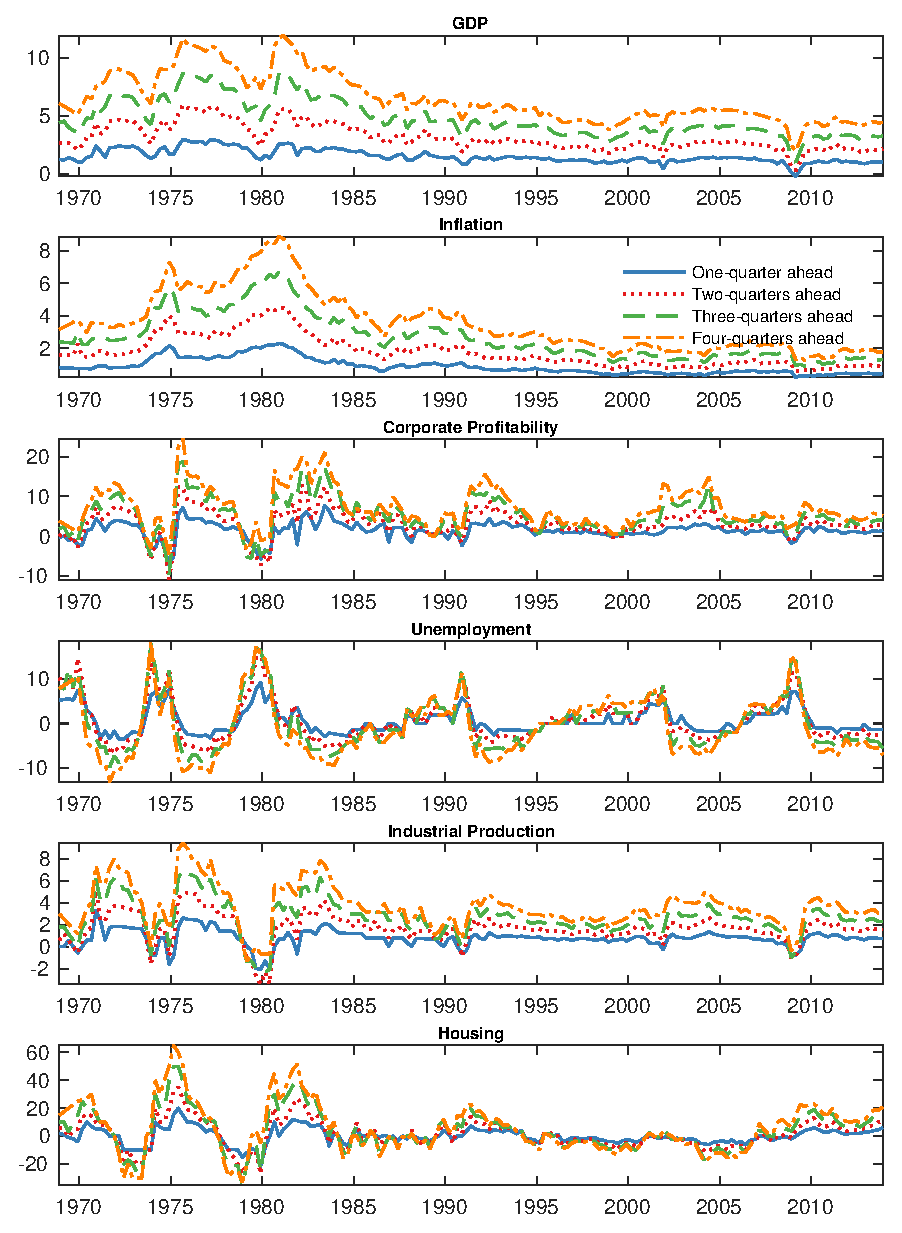
\includegraphics[scale=0.8]{figures/e_survey_expectations.eps}
    \label{Fig:e_survey_expectations}
\end{figure}
As a verification, we plot in Figure \ref{Fig:e_survey_expectations} one- through four-quarter ahead forecasts from the SPF. As suggested by the descriptive statistics, we see that the majority of the forecasts are indeed displaying extrapolative behavior.

%----------------------------------------------------------------------------------------------------------------------
% VISUALIZING PRINCIPAL COMPONENT LOADINGS
%----------------------------------------------------------------------------------------------------------------------

\clearpage
\section{Visualizing principal component loadings}\label{sec:visualizing_principal_component_loaings}
While the loadings from the principal component analysis are tabulated in Table \ref{Tab:e_sumstat_survey_variables}, this section provides a visual interpretation by plotting the loadings in bar form in Figure \ref{Fig:e_pca_loadings}.
\begin{figure}[htbp]
    \caption{
        \textbf{Principal component loadings.} \newline
        This figure illustrates the loadings from the principal component analysis in Section \ref{Sec:e_measuring_ebc}. Loadings are grouped by macroeconomic fundamentals and ordered from shortest to longest forecast horizon. 
    }
    \centering
    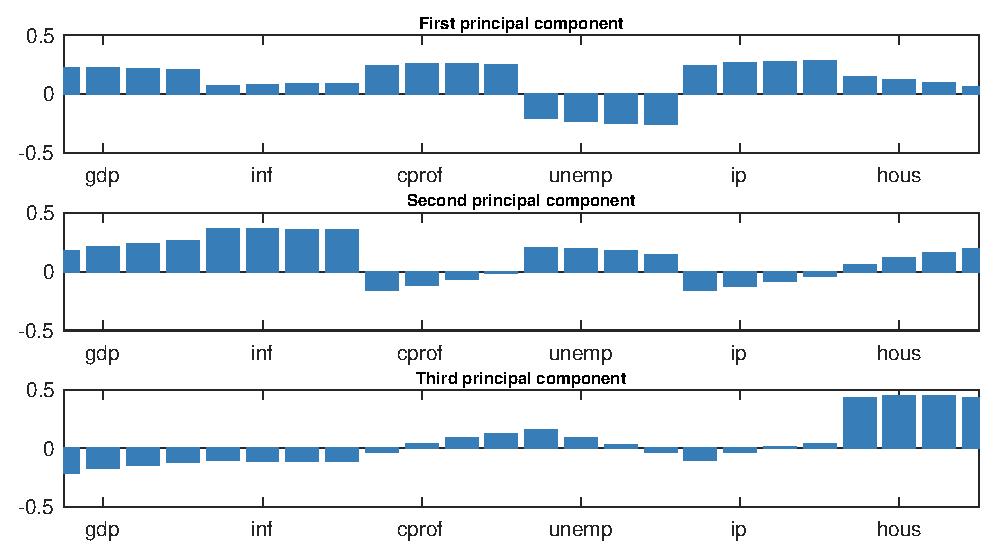
\includegraphics[scale=0.8]{figures/e_pca_loadings.eps}
    \label{Fig:e_pca_loadings}
\end{figure}
The interpretation is naturally identical to the one obtained from the tabulated loadings, but the visualization may be more informative in some aspects. In particular, the graphical illustration naturally revels that loadings are similar in size for a particular fundamental across forecast horizons, albeit some heterogeneity in loading sizes are present. However, no loading is placed entirely on a particular forecast horizon for any of the macroeconomic fundamentals. 

%----------------------------------------------------------------------------------------------------------------------
% PLOTTING PCA LOADINGS
%----------------------------------------------------------------------------------------------------------------------

\clearpage
\section{Participation of individual forecasters}\label{sec:e_participation_of_individual_forecasters}
As mentioned in Section \ref{Sec:e_measuring_ebc}, the average number of participating forecasters in our sample is about $36$ per quarter. However, this number fluctuates over time as individual forecasters exit and enter the sample at various points in time.\footnote{See \cite{CapistranTimmermann2009} for a discussion on how best to deal with these exits and entries from a forecasting perspective.} To illustrate the participation, we consider in Figure \ref{Fig:e_participating_forecasters} the one-quarter ahead forecasts provided for the GDP variable over our sample period. 
\begin{figure}[htbp]
    \caption{
        \textbf{Participation of individual forecasters.} \newline
        This figure illustrates the participation of individual forecasters over our sample period. The blue dots represents a submitted forecasts from forecaster $i$ at time $t$. Forecaster IDs with no forecast submissions have been removed for easier readability of the figure. As a result, our notation of Forecaster ID need not correspond to the ID from the Survey of Professional Forecasters (SPF). The sample period starts in 1968:Q4 and ends in 2014:Q4.
    }
    \centering
    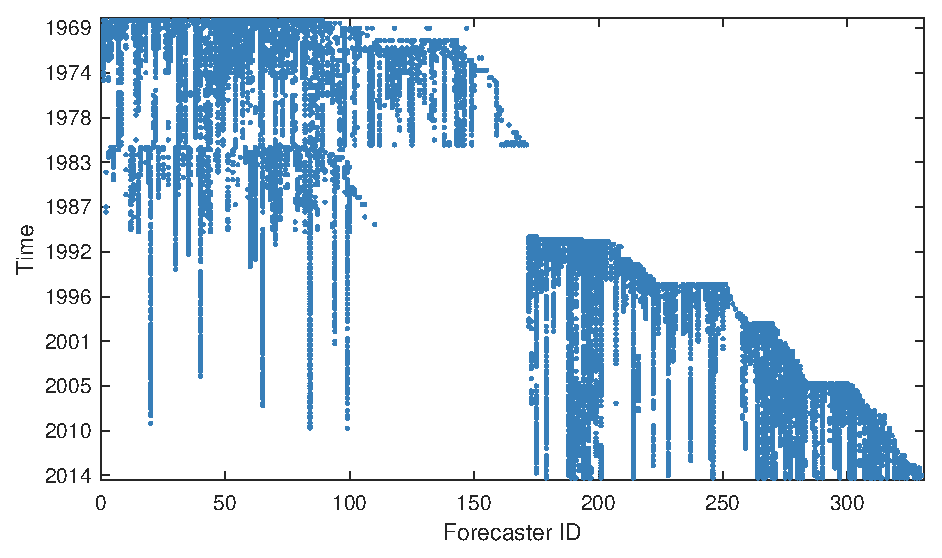
\includegraphics[scale=0.8]{figures/e_participating_forecasters.eps}
    \label{Fig:e_participating_forecasters}
\end{figure}
Each dot represents a response by forecaster $i$, who are represented by a unique, but anonymous, forecaster ID, at time $t$. We see that the composition of the panel of professional forecasters vary over time and that individual forecasters frequently enter, exit, and re-enter the sample at various points in time. 

\end{appendices}
\end{document}

%----------------------------------------------------------------------------------------------------------------------
% END OF DOCUMENT
%----------------------------------------------------------------------------------------------------------------------